% !TEX root = Tese_LucasMaio.tex
\documentclass[12pt, openany]{report}
% \documentclass[12pt,showframe, openleft]{report}

%%%%%%%%%%%%%%%%%%%%%%%%%%%%%%%%%%%%%%%%%%%%%%%%%%%%%%%%%%%%%%%%%%%%%%%%%%%%%%%%
% TEMPLATE PARA DOCUMENTOS
% UFABC Rocket Design
% 
% Lista de revisões: (data ISO - nome)
% 
% 2020-12-17 - Heitor Rodrigues Savegnago
% 2021-01-17 - Heitor Rodrigues Savegnago
% 2021-01-23 - Heitor Rodrigues Savegnago
% 2021-04-21 - Heitor Rodrigues Savegnago
% 2021-12-23 - Heitor Rodrigues Savegnago
% 2022-02-02 - Heitor Rodrigues Savegnago
% 2022-04-19 - Heitor Rodrigues Savegnago
% 2022-11-02 - Heitor Rodrigues Savegnago
% 2023-05-24 - Heitor Rodrigues Savegnago
% 2023-08-06 - Heitor Rodrigues Savegnago
% 2023-08-18 - Heitor Rodrigues Savegnago
% 2023-09-06 - Heitor Rodrigues Savegnago
% 2023-09-27 - Heitor Rodrigues Savegnago
% 
%%%%%%%%%%%%%%%%%%%%%%%%%%%%%%%%%%%%%%%%%%%%%%%%%%%%%%%%%%%%%%%%%%%%%%%%%%%%%%%% 

% Formatação geral do documento

    % Configuração de margens
    \ifx\standalone\undefined
        \usepackage[a4paper, twoside, top = 3cm, bottom = 2cm, left = 3cm, right = 2cm]{geometry} % Margens do documento
    \fi

    % Fonte
        %\renewcommand{\rmdefault}{phv} % Arial
        \usepackage[lighttt]{lmodern} % Fonte Latin Modern
        % \renewcommand{\familydefault}{\sfdefault} % Estilo global Sans Serif
        
    % Espaçamento entre linhas
        \usepackage{setspace} % Espaçamento do texto
        	\renewcommand{\baselinestretch}{1.15}
    
    % Correções de espaçamentos
        \usepackage{indentfirst} % Parágrafos indentados
        	\setlength{\parindent}{1cm} % Define espaço de paragrafo como 1cm
        	
        \raggedbottom % Corrige espaçamento de paragrafo
    
    % Decorações da página
        \usepackage{fancyhdr} % Cabeçalhos e rodapés em páginas
    
    % Formatação de títulos
    	\newcommand{\titlefont}{\fontsize{18}{20}}
    	\newcommand{\sectionfont}{\fontsize{16}{20}}
    	\newcommand{\subsectionfont}{\fontsize{14}{20}}
    	\newcommand{\subsubsectionfont}{\fontsize{12}{20}}
    	
        \usepackage{titlesec} % Configurações para seção
            \titleformat{\chapter}{\normalfont \titlefont \bfseries}{\thechapter}{1em}{}
            \titleformat{\section}{\normalfont \sectionfont \bfseries}{\thesection}{1em}{}
            \titleformat{\subsection}{\normalfont \subsectionfont \bfseries}{\thesubsection}{1em}{}
            \titleformat{\subsubsection}{\normalfont \subsubsectionfont \bfseries}{\thesubsubsection}{1em}{}
            \titlespacing*{\chapter}{0pt}{3.5ex plus 1ex minus .2ex}{2.3ex plus .2ex}
        	
        \usepackage{titletoc} % Configurações para seção no sumário
            % \contentsmargin{2.55em}
            \dottedcontents{chapter}[4em]{\vspace{1em}\bfseries}{4em}{0.4em}

% \titlecontents{chapter}
% [4em] % ie, 1.5em (chapter) + 2.3em
% {}
% {\MakeUpper\contentslabel{2.3em}}
% {\MakeUpper\hspace*{-2.3em}}
% {\titlerule*[1pc]{.}\contentspage}

% \titlecontents{chapter}[2em]
%     {\vspace{12pt}}
%     {\normalfont\normalsize\contentslabel[\thecontentslabel.0]{2em}\uppercase}
%     {\hspace*{-2em}\uppercase}
%     {\titlerule*[.75em]{.}\contentspage}

            
            \dottedcontents{section}[4em]{\bfseries}{4em}{0.4em}
            \dottedcontents{subsection}[4em]{}{4em}{0.4em}
            \dottedcontents{subsubsection}[4em]{}{4em}{0.4em}
        
    % Alteração de limite de níveis no sumário
        
        \setcounter{tocdepth}{4} % Níveis exibidos no sumário
        \setcounter{secnumdepth}{4} % Nível de números exibidos
        
    % Opções para tópicos de enumerate
    
        \usepackage[shortlabels]{enumitem} % Selecionar formato em itemize

%%%%%%%%%%%%%%%%%%%%%%%%%%%%%%%%%%%%%%%%%%%%%%%%%%%%%%%%%%%%%%%%%%%%%%%%%%%%%%%%

% Codificação de carecteres de entrada

    \usepackage{ae} % "Almost European"
    \usepackage[T1]{fontenc} % Caracteres especiais
    \usepackage[utf8]{inputenc} % Caracteres especiais

%%%%%%%%%%%%%%%%%%%%%%%%%%%%%%%%%%%%%%%%%%%%%%%%%%%%%%%%%%%%%%%%%%%%%%%%%%%%%%%%

% Configuração de linguagem padrão do documento

    \usepackage[brazil]{babel} % Detalhes automáticos em Português
	
	\AtBeginDocument{\renewcommand{\contentsname}{\centerline{Sumário}}}
	\AtBeginDocument{\renewcommand{\bibname}{Referências Bibliográficas}}
% 	\AtBeginDocument{\renewcommand{\figurename}{Figura}}
% 	\AtBeginDocument{\renewcommand{\tablename}{Tabela}}

    \usepackage{textcomp} % Suporte de caracteres especiais

    \usepackage{csquotes} % Opções de citação

%%%%%%%%%%%%%%%%%%%%%%%%%%%%%%%%%%%%%%%%%%%%%%%%%%%%%%%%%%%%%%%%%%%%%%%%%%%%%%%%

% Configurações de core

    \usepackage{transparent}

    \usepackage[svgnames]{xcolor}%Define cores

        \definecolor{0DF}{HTML}{00DDFF}
        \definecolor{0FD}{HTML}{00FFDD}
        \definecolor{DF0}{HTML}{DDFF00}
        \definecolor{FD0}{HTML}{FFDD00}
        \definecolor{F0D}{HTML}{FF00DD}
        \definecolor{D0F}{HTML}{DD00FF}
        
        \definecolor{0BD}{HTML}{00BBDD}
        \definecolor{0DB}{HTML}{00DDBB}
        \definecolor{BD0}{HTML}{BBDD00}
        \definecolor{DB0}{HTML}{DDBB00}
        \definecolor{D0B}{HTML}{DD00BB}
        \definecolor{B0D}{HTML}{BB00DD}
        
        \definecolor{09B}{HTML}{0099BB}
        \definecolor{0B9}{HTML}{00BB99}
        \definecolor{9B0}{HTML}{99BB00}
        \definecolor{B90}{HTML}{BB9900}
        \definecolor{B09}{HTML}{BB0099}
        \definecolor{90B}{HTML}{9900BB}
        
        \definecolor{079}{HTML}{007799}
        \definecolor{097}{HTML}{009977}
        \definecolor{790}{HTML}{779900}
        \definecolor{970}{HTML}{997700}
        \definecolor{907}{HTML}{990077}
        \definecolor{709}{HTML}{770099}
        
        \definecolor{057}{HTML}{005577}
        \definecolor{075}{HTML}{007755}
        \definecolor{570}{HTML}{557700}
        \definecolor{750}{HTML}{775500}
        \definecolor{705}{HTML}{770055}
        \definecolor{507}{HTML}{550077}
        
        \definecolor{035}{HTML}{003355}
        \definecolor{053}{HTML}{005533}
        \definecolor{350}{HTML}{335500}
        \definecolor{530}{HTML}{553300}
        \definecolor{503}{HTML}{550033}
        \definecolor{305}{HTML}{330055}
        
        \definecolor{013}{HTML}{001133}
        \definecolor{031}{HTML}{003311}
        \definecolor{130}{HTML}{113300}
        \definecolor{310}{HTML}{331100}
        \definecolor{301}{HTML}{330011}
        \definecolor{103}{HTML}{110033}
        
        \definecolor{strs}			{rgb}	{0.9,	0.2,	0	}
        \definecolor{coments}		{rgb}	{0,		0.5,	0	} 
        \definecolor{backcode}		{rgb}	{0.3,	0,		0.2	}
        
        \newcommand{\MexerDepois}[1]{{\huge\color{F0D}#1}}
        \newcommand{\mexer}[1]{{\color{F0D}#1}}
        
        \newcommand{\showcolors}%Mostra tabela de cores
        {{\ttfamily
        		{\color{0DF}$\overset{\text{\tiny 0DF}}{\blacksquare}$}
        		{\color{0BD}$\overset{\text{\tiny 0BD}}{\blacksquare}$}
        		{\color{09B}$\overset{\text{\tiny 09B}}{\blacksquare}$}
        		{\color{079}$\overset{\text{\tiny 079}}{\blacksquare}$}
        		{\color{057}$\overset{\text{\tiny 057}}{\blacksquare}$}
        		{\color{035}$\overset{\text{\tiny 035}}{\blacksquare}$}
        		{\color{013}$\overset{\text{\tiny 013}}{\blacksquare}$}
        		\\
        		{\color{0FD}$\overset{\text{\tiny 0FD}}{\blacksquare}$}
        		{\color{0DB}$\overset{\text{\tiny 0DB}}{\blacksquare}$}
        		{\color{0B9}$\overset{\text{\tiny 0B9}}{\blacksquare}$}
        		{\color{097}$\overset{\text{\tiny 097}}{\blacksquare}$}
        		{\color{075}$\overset{\text{\tiny 075}}{\blacksquare}$}
        		{\color{053}$\overset{\text{\tiny 053}}{\blacksquare}$}
        		{\color{031}$\overset{\text{\tiny 031}}{\blacksquare}$}
        		\\
        		{\color{DF0}$\overset{\text{\tiny DF0}}{\blacksquare}$}
        		{\color{BD0}$\overset{\text{\tiny BD0}}{\blacksquare}$}
        		{\color{9B0}$\overset{\text{\tiny 9B0}}{\blacksquare}$}
        		{\color{790}$\overset{\text{\tiny 790}}{\blacksquare}$}
        		{\color{570}$\overset{\text{\tiny 570}}{\blacksquare}$}
        		{\color{350}$\overset{\text{\tiny 350}}{\blacksquare}$}
        		{\color{130}$\overset{\text{\tiny 130}}{\blacksquare}$}
        		\\
        		{\color{FD0}$\overset{\text{\tiny FD0}}{\blacksquare}$}
        		{\color{DB0}$\overset{\text{\tiny DB0}}{\blacksquare}$}
        		{\color{B90}$\overset{\text{\tiny B90}}{\blacksquare}$}
        		{\color{970}$\overset{\text{\tiny 970}}{\blacksquare}$}
        		{\color{750}$\overset{\text{\tiny 750}}{\blacksquare}$}
        		{\color{530}$\overset{\text{\tiny 530}}{\blacksquare}$}
        		{\color{310}$\overset{\text{\tiny 310}}{\blacksquare}$}
        		\\
        		{\color{F0D}$\overset{\text{\tiny F0D}}{\blacksquare}$}
        		{\color{D0B}$\overset{\text{\tiny D0B}}{\blacksquare}$}
        		{\color{B09}$\overset{\text{\tiny B09}}{\blacksquare}$}
        		{\color{907}$\overset{\text{\tiny 907}}{\blacksquare}$}
        		{\color{705}$\overset{\text{\tiny 705}}{\blacksquare}$}
        		{\color{503}$\overset{\text{\tiny 503}}{\blacksquare}$}
        		{\color{301}$\overset{\text{\tiny 301}}{\blacksquare}$}
        		\\
        		{\color{D0F}$\overset{\text{\tiny D0F}}{\blacksquare}$}
        		{\color{B0D}$\overset{\text{\tiny B0D}}{\blacksquare}$}
        		{\color{90B}$\overset{\text{\tiny 90B}}{\blacksquare}$}
        		{\color{709}$\overset{\text{\tiny 709}}{\blacksquare}$}
        		{\color{507}$\overset{\text{\tiny 507}}{\blacksquare}$}
        		{\color{305}$\overset{\text{\tiny 305}}{\blacksquare}$}
        		{\color{103}$\overset{\text{\tiny 103}}{\blacksquare}$}
        }}

%%%%%%%%%%%%%%%%%%%%%%%%%%%%%%%%%%%%%%%%%%%%%%%%%%%%%%%%%%%%%%%%%%%%%%%%%%%%%%%%

% Configurações do pacote listings para adição de código no documento

    \usepackage{listings}%Configura layout para mostrar codigos a partir de arquivo
        \AtBeginDocument{\renewcommand{\lstlistingname}{Código}}

        
        \lstdefinelanguage{JavaScript}{
            keywords={typeof, new, true, false, catch, function, return, null, catch, switch, var, if, in, while, do, else, case, break},
            ndkeywords={class, export, boolean, throw, implements, import, this},
            % ndkeywordstyle=\color{darkgray}\bfseries,
            identifierstyle=\color{black},
            sensitive=false,
            comment=[l]{//},
            morecomment=[s]{/*}{*/},
            morestring=[b]',
            morestring=[b]"
        }
        
        \lstset{% Configurando layout para mostrar códigos C++
            language=[11]C++,
            basicstyle=\ttfamily\small\setstretch{1},
            backgroundcolor=\color{backcode!5},
            stringstyle=\color{strs}, 
            commentstyle=\color{coments},
            keywordstyle=[1]\itshape\color{079}, 
            keywordstyle=[2]\color{907},
            keywordstyle=[3]\color{097},
            keywordstyle=[4]\bfseries\color{790},
            keywordstyle=[5]\color{709},
            keywordstyle=[6]\color{970},
            morekeywords=[1]{byte},
            morekeywords=[2]{},
            morekeywords=[3]{uint8_t, size_t, type},
            morekeywords=[4]{},
            numbers=left,
            numberstyle=\tiny,
            escapeinside={§}{§},
            tabsize=2,
            extendedchars=true, 
            showspaces=false, 
            showstringspaces=false, 
            numberbychapter=false,
            emptylines=1,
            frame=L,
            firstnumber=auto,
            breaklines=true,
            breakautoindent=true, 
            captionpos=t,
            float=htbp, 
            xleftmargin=2em,
            inputencoding=utf8,
            %texcl=true,
            upquote=true,
            literate=%
                {á}{{\'a}}1 {à}{{\`a}}1 {â}{{\^a}}1 {ä}{{\"a}}1 {ã}{{\~a}}1
                {Á}{{\'A}}1 {À}{{\`A}}1 {Â}{{\^A}}1 {Ä}{{\"A}}1 {Ã}{{\~A}}1
                {é}{{\'e}}1 {è}{{\`e}}1 {ê}{{\^e}}1 {ë}{{\"e}}1
                {É}{{\'E}}1 {È}{{\`E}}1 {Ê}{{\^E}}1 {Ë}{{\"E}}1
                {í}{{\'i}}1 {ì}{{\`i}}1 {î}{{\^i}}1 {ï}{{\"i}}1
                {Í}{{\'I}}1 {Ì}{{\`I}}1 {Î}{{\^I}}1 {Ï}{{\"I}}1
                {ó}{{\'o}}1 {ò}{{\`o}}1 {ô}{{\^o}}1 {ö}{{\"o}}1 {õ}{{\~o}}1
                {Ó}{{\'O}}1 {Ò}{{\`O}}1 {Ô}{{\^O}}1 {Ö}{{\"0}}1 {Õ}{{\~O}}1
                {ú}{{\'u}}1 {ù}{{\`u}}1 {û}{{\^u}}1 {ü}{{\"u}}1
                {Ú}{{\'U}}1 {Ù}{{\`U}}1 {Û}{{\^U}}1 {Ü}{{\"U}}1
                {ç}{{\c{c}}}1 {Ç}{{\c{C}}}1
                {°}{{\textdegree}}1
                {¹}{{\textsuperscript{1}}}1
                {²}{{\textsuperscript{2}}}1
                {³}{{\textsuperscript{3}}}1
        }
        
        \newcommand{\coda}[1]{{\color{057}\lstinline|#1|}}
        \newcommand{\code}[1]{{\color{075}\lstinline|#1|}}
        \newcommand{\codi}[1]{{\color{570}\lstinline|#1|}}
        \newcommand{\codo}[1]{{\color{750}\lstinline|#1|}}
        \newcommand{\codu}[1]{{\color{705}\lstinline|#1|}}
        \newcommand{\codw}[1]{{\color{507}\lstinline|#1|}}
        \newcommand{\codGuide}{
            \begin{center}
                \large{\coda{A}\\\code{E}\\\codi{I}\\\codo{O}\\\codu{U}\\\codw{W}
                
                \showcolors}
            \end{center}
        }

%%%%%%%%%%%%%%%%%%%%%%%%%%%%%%%%%%%%%%%%%%%%%%%%%%%%%%%%%%%%%%%%%%%%%%%%%%%%%%%%

% Adição de caracteres

    \usepackage[euler]{textgreek} % Caracteres gregos

    \usepackage{pmboxdraw} % Caracteres unicode 

%%%%%%%%%%%%%%%%%%%%%%%%%%%%%%%%%%%%%%%%%%%%%%%%%%%%%%%%%%%%%%%%%%%%%%%%%%%%%%%%

% Pacotes de opções matemáticas

    \usepackage{amsmath, amssymb, xfrac, cancel} % símbolos matemáticos
    
    \usepackage{siunitx} % Comando \SI para unidades de medida
        \sisetup{locale = FR} % Utilizar virgular para marcação decimal
        \sisetup{separate-uncertainty = true}
        \sisetup{exponent-product=\ensuremath{\cdot}}
        \sisetup{separate-uncertainty=true}
        \sisetup{multi-part-units=single}
        \sisetup{group-separator = {}}
        
        \DeclareSIUnit{\nothing}{{\relax}}
        \DeclareSIUnit{\var}{VAR}
        \DeclareSIUnit{\va}{VA}
        \DeclareSIUnit{\dBm}{dBm}
        
    \usepackage{gensymb} % Símbolos de unidades de medida
    
    \usepackage{mathtools}

        \DeclareFontFamily{U}{mathc}{}
        \DeclareFontShape{U}{mathc}{m}{it}%
        {<->s*[1.03] mathc10}{}
        \DeclareMathAlphabet{\mathcal}{U}{mathc}{m}{it}
        
        \DeclareMathOperator{\sHom}{\mathcal{H\mkern-3mu om}}
        \DeclareMathOperator{\sExt}{\mathcal{E\mkern-3mu xt}}
        \DeclareMathOperator{\sEnd}{\mathcal{E\mkern-3mu nd}}

    \usepackage{steinmetz} % Números complexos

%%%%%%%%%%%%%%%%%%%%%%%%%%%%%%%%%%%%%%%%%%%%%%%%%%%%%%%%%%%%%%%%%%%%%%%%%%%%%%%%

% Pacotes de opções químicas

    \usepackage{chemformula}
    \usepackage[version=3]{mhchem}
    
%%%%%%%%%%%%%%%%%%%%%%%%%%%%%%%%%%%%%%%%%%%%%%%%%%%%%%%%%%%%%%%%%%%%%%%%%%%%%%%%

% Opções adicionais para formatação

    \usepackage[normalem]{ulem} % Sublinados diversos
    
    \usepackage{framed} % Criar caixas inteligentes
    
    \usepackage{footnote} % Notas de rodapé

    \usepackage{lscape} % Página em paisagem

%%%%%%%%%%%%%%%%%%%%%%%%%%%%%%%%%%%%%%%%%%%%%%%%%%%%%%%%%%%%%%%%%%%%%%%%%%%%%%%%

% Formatação de tabelas

    \usepackage{tabularx} % Tabelas do tipo tabularx
    \usepackage{booktabs} % Formatação de tabelas como em livro
        %\renewcommand{\arraystretch}{2} % Espaçamento entre linhas interno em tabelas
        %\renewcommand{\cellgape}{\Gape[4pt]} % Espaçamento de tabelas
    \usepackage{makecell} % formatação avançada para tabelas
    \usepackage{multirow} % Merge em tabelas
    \usepackage{multicol} % Texto em colunas na folha
    \usepackage{arydshln} % Draw dash-lines in array/tabular
    \usepackage{colortbl} % Linhas, colunas e celulas coloridas
    
    \usepackage{array} % opções especiais para alinhamento de tabelas
    {
        \newcolumntype{L}[1]{>{\raggedright\let\newline\\\arraybackslash\hspace{0pt}}m{#1}}
        \newcolumntype{C}[1]{>{\centering\let\newline\\\arraybackslash\hspace{0pt}}m{#1}}
        \newcolumntype{R}[1]{>{\raggedleft\let\newline\\\arraybackslash\hspace{0pt}}m{#1}}
    }

%%%%%%%%%%%%%%%%%%%%%%%%%%%%%%%%%%%%%%%%%%%%%%%%%%%%%%%%%%%%%%%%%%%%%%%%%%%%%%%%

% Pacotes para trabalhar com figuras

    \usepackage{graphicx} % Adição de imagens
    
    \usepackage{svg} % Adição de imagens no formato SVG

    \usepackage[outdir=./]{epstopdf} % Figuras em EPS convertidas em PDF
    
    \usepackage{pdfpages} % Adição de PDFs como páginas
    
    \usepackage{tikz} % Desenhos
        \usetikzlibrary{through,shapes}
        \usetikzlibrary{trees}
        \usetikzlibrary{fit}
        \usetikzlibrary{patterns}
        \usetikzlibrary{calc}
        \usetikzlibrary{arrows,decorations,decorations.pathmorphing,positioning}
    
    \usepackage{pgfplots} % Desenho de gráficos
        \pgfdeclarelayer{background}    % declare background layer
        \pgfdeclarelayer{foreground}    % declare foreground layer
        \pgfsetlayers{background,main,foreground}  % set the order of the layers (main is the standard layer)
        \pgfplotsset{compat=1.14}
        \usepgfplotslibrary{fillbetween}
        
    \usepackage{pgf-pie} % Gráficos pizza
    
    \usepackage[RPvoltages]{circuitikz} % Desenhos de circuitos
        \ctikzset{bipoles/thickness=1}
        
    
    \usepackage{chemfig} % Desenho de moléculas

%%%%%%%%%%%%%%%%%%%%%%%%%%%%%%%%%%%%%%%%%%%%%%%%%%%%%%%%%%%%%%%%%%%%%%%%%%%%%%%%

% Utilitários adicionais para lidar com figuras e tabelas

    \usepackage{float} % posicionamento espacial

        % Criando ambiente float para códigos
        \newfloat{lstfloat}{htbp}{lop}
        \floatname{lstfloat}{Código}
        \def\lstfloatautorefname{Código} % needed for hyperref/auroref
    
    \usepackage{caption} % Comando \caption*
    
    \usepackage{subcaption} % Opções de subfiguras

%%%%%%%%%%%%%%%%%%%%%%%%%%%%%%%%%%%%%%%%%%%%%%%%%%%%%%%%%%%%%%%%%%%%%%%%%%%%%%%%

% Referência cruzada e links
    
    \usepackage[hidelinks]{hyperref} % Links no documento
    
    \usepackage{nameref} % Referenciar entidades por nome

    \usepackage{titleref} % Referenciar títulos

%%%%%%%%%%%%%%%%%%%%%%%%%%%%%%%%%%%%%%%%%%%%%%%%%%%%%%%%%%%%%%%%%%%%%%%%%%%%%%%%

% Configuração de contadores do documento

    \ifx\letter\undefined
    \usepackage{chngcntr} % Muda os contadores de figuras, equações, etc
        \counterwithout{figure}{chapter} % Número de figura sem contar capítulo
        \counterwithout{table}{chapter} % Número de tabela sem contar capítulo
        \counterwithout{equation}{chapter} % Número de equação sem contar capítulo
    \fi
%%%%%%%%%%%%%%%%%%%%%%%%%%%%%%%%%%%%%%%%%%%%%%%%%%%%%%%%%%%%%%%%%%%%%%%%%%%%%%%%

% controle de citação e referências bibliográfica

    \usepackage[backend=biber, style=ieee, citestyle=numeric, sorting=none]{biblatex}
    % \usepackage[style=abnt-numeric, citestyle=numeric, sorting=none]{biblatex} %https://github.com/abntex/biblatex-abnt/issues/90
    
%%%%%%%%%%%%%%%%%%%%%%%%%%%%%%%%%%%%%%%%%%%%%%%%%%%%%%%%%%%%%%%%%%%%%%%%%%%%%%%%

% Auxiliares gerais

    \usepackage{lipsum} % Lorem ipsum

    \usepackage{ifdraft} % Opções adicionais para o modo draft

    \usepackage{etoolbox} % Toolbox of programming facilities
    
%%%%%%%%%%%%%%%%%%%%%%%%%%%%%%%%%%%%%%%%%%%%%%%%%%%%%%%%%%%%%%%%%%%%%%%%%%%%%%%%

% Definições de macros especiais para capa e folha de rosto

    % Lista de nomes
    
        \newcommand{\name}[1]
        {
        	&{#1}\\
        }
        \newenvironment{names}[1]
        {
            \begin{table}[H]\flushleft
        		\begin{tabular}{>{\raggedleft}p{.45\linewidth} | >{\bf}p{.45\linewidth}}
        			\sf{#1}
        			}
                    	%args here
                    {
        		\end{tabular}
        	\end{table}
        }

    % Outras macros
        \providecommand{\keywords}[1]{\textbf{{Keywords:}} #1}
        \providecommand{\palavraschave}[1]{\textbf{{Palavras-chave:}} #1}

    \newcommand{\nomes}{}
    \newcommand{\grupo}{}
    \newcommand{\centro}{}
    \newcommand{\centroSigla}{}
    \newcommand{\disciplina}{}
    \newcommand{\codigoDisciplina}{}
    \newcommand{\titulo}{}
    \newcommand{\professor}{}
    \newcommand{\local}{}
    \newcommand{\data}{}
    \newcommand{\notaDeRosto}{}
    \newcommand{\cabecalho}
    {
        {\large%
        \textbf{UNIVERSIDADE FEDERAL DO ABC}}\\
        \expandafter\MakeUppercase\expandafter{\small\centro{}%
        \ifdefempty{\centro}{}{ - }%
        \centroSigla\\
        \codigoDisciplina{}%
        \ifdefempty{\codigoDisciplina}{}{ - }%
        \disciplina%
        }
    }
    
    \newcommand{\capaComLogo}{
        \begin{titlepage} \center
            \cabecalho
            
            \vspace{6em}
            
            \begin{center}
                
\includegraphics[width=0.335\linewidth]{pictures/logo_ufabc}
            \end{center}
            
            \nomes
            \textbf{\grupo} 
            
            \vfill
            
            {\large{\MakeUppercase{\textbf{\titulo}}}}
            
            \vspace{1.5cm}
    		\professor
      
    		\vfill
    		\vfill
            
    		{\local\\\data}
        \end{titlepage}
    }
    
    \newcommand{\capa}{
        \begin{titlepage} \center
            \cabecalho
            
            \vspace{6em}
            
            % \capaLogo
            
            \nomes
            
            \vfill
            
            {\large{\MakeUppercase{\textbf{\titulo}}}}
            
            % \\\vspace{1.5cm}
    		% \professor
      
    		\vfill
    		\vfill
            
    		{\local\\\data}
        \end{titlepage}
    }
    
    \newcommand{\folhaDeRosto}{
        \newpage
        \begin{titlepage}
    		\center
            \nomes
            % \vspace{5cm}
            \vfill
            {\large{\MakeUppercase{\textbf{\titulo}}}}
            \vfill
            \hfill\begin{minipage}{0.5\linewidth}\onehalfspacing
            \notaDeRosto
            \end{minipage}
            \vfill
    		{\local\\\data}
        \end{titlepage}
    }

%%%%%%%%%%%%%%%%%%%%%%%%%%%%%%%%%%%%%%%%%%%%%%%%%%%%%%%%%%%%%%%%%%%%%%%%%%%%%%%%

% Configurações de estilos de páginas

\AtBeginDocument{%
    %
    \ifx\standalone\undefined
        \setlength{\headheight}{1.5em}
    \else
        \fancyhf{}
        \renewcommand{\headrulewidth}{0pt}
	    \pagestyle{plain}
    \fi
    %
	\titleformat{\chapter}{\normalfont \titlefont \bfseries}{\chaptername\ \thechapter}{1em}{}
	% \titleformat{\chapter}{\normalfont \titlefont \bfseries}{\thechapter}{1em}{}
	%
    \renewcommand{\chaptermark}[1]{\markboth{#1}{}} %mostrar somente o nome do capítulo com \leftmark
    %
    \pagestyle{fancy}
    \fancypagestyle{plain}{% Página padrão
        \renewcommand{\headrulewidth}{0pt}
	    % \pagenumbering{arabic}
    }
    \fancypagestyle{main}{% Página padrão
        \fancyhf{}
        \lhead{}
        \chead{}
        \rhead{}
        \lfoot{}
        \cfoot{\thepage}
        \rfoot{}
	    \pagenumbering{arabic}
    }
    %
    \fancypagestyle{toc}{% Página  do sumário
        \renewcommand{\headrulewidth}{0pt}
        \fancyhf{}
        \lhead{}
        \chead{}
        \rhead{}
        \lfoot{}
        \cfoot{\thepage}
        \rfoot{}
	    \pagenumbering{Roman}
    }
    %
    \fancypagestyle{clear}{% Página do sumário
        \fancyhf{}
        \lhead{}
        \chead{}
        \rhead{}
        \lfoot{}
        \cfoot{}
        \rfoot{}
	   % \pagenumbering{None}
    }
    %
    \fancypagestyle{letterCapitania}{% Página do modelo de carta
        \fancyhf{}
        \renewcommand{\headrulewidth}{0pt}
	    \setlength\headheight{70pt}
        \lhead{
            \textbf{Carta de Intenções}\\
            \textbf{\today}\\\vspace{1em}
            Chapa: \chapa
            \vfill}
        \chead{}
        \rhead{\includegraphics[height=0.925\headheight]{Templates/logo_rocket.eps}}
        \lfoot{}
        \cfoot{\thepage}
        \rfoot{}
	    \pagenumbering{arabic}
    }
}

%%%%%%%%%%%%%%%%%%%%%%%%%%%%%%%%%%%%%%%%%%%%%%%%%%%%%%%%%%%%%%%%%%%%%%%%%%%%%%%%
% !TEX root = ../raiz.tex

% http://bcc.ufabc.edu.br/documentos/normalizacao.pdf

\renewcommand{\nomes}
{
	\begin{table}[H]
		\centering
		\begin{tabular}{ll}
			
			Lucas Maio Nunes de Almeida Gonçalves & 11201721618 \\
            
		\end{tabular}
	\end{table}
}

\renewcommand{\centro}{Centro de Engenharia, Modelagem e Ciências Sociais Aplicadas}
\renewcommand{\centroSigla}{CECS}
% \renewcommand{\centro}{Centro de Ciências Naturais e Humanas}
% \renewcommand{\centroSigla}{CCNH}
% \renewcommand{\centro}{Centro de Matemática, Computação e Cognição}
% \renewcommand{\centroSigla}{CMCC}

\renewcommand{\disciplina}{Trabalho de Graduação III em Engenharia Biomédica}
\renewcommand{\codigoDisciplina}{ESTI902-17}

% \renewcommand{\disciplina}{Projeto de Graduação em Computação I}
% \renewcommand{\codigoDisciplina}{MCTA029-17}

\renewcommand{\titulo}{Desenvolvimento de Interface PyQt para Controle de Parâmetros em Tomografia por Impedância Elétrica usando pyEIT.}

% \renewcommand{\professor}{Prof. Dr. Francisco de Assis Zampirolli}
\renewcommand{\professor}{Orientado por: Prof. Dr. Erick Dario Leon Bueno de Camargo}

\renewcommand{\local}{São Bernardo, SP}

\renewcommand{\data}{2026}

\renewcommand{\notaDeRosto}
{
    \singlespacing
    Trabalho de Conclusão de Curso apresentado ao \centro{} 
    da Universidade Federal do ABC como requisito parcial 
    à obtenção do título de Bacharel em Engenharia Biomédica.
    
    \vspace{1em}
    
    Orientador: Prof. Dr. Erick Dario Leon Bueno de Camargo.
} 


\bibliography{reference.bib}

\begin{document}

    \capaComLogo
    \folhaDeRosto    
    % \folhaDeAprovacao
    \pagestyle{toc}
    % !TEX root = ../Tese_LucasMaio.tex

\chapter*{Resumo}

A Tomografia por Impedância Elétrica (TIE) é uma técnica de imageamento funcional não invasiva, portátil e livre de radiação ionizante, cuja reconstrução depende de métodos numéricos e de escolhas de visualização que influenciam diretamente a interpretação das imagens. Neste trabalho, foi desenvolvida uma interface gráfica interativa, em Python, voltada à reconstrução e visualização de dados previamente registrados de TIE, com foco educacional e de apoio à pesquisa. A aplicação integrou o framework \textit{open-source} pyEIT a uma arquitetura modular inspirada no padrão MVC (\textit{Model--View--Controller}) e incorporou três métodos de reconstrução --- Back-Projection (BP), Jacobiano (JAC) e GREIT --- além de duas implementações de interface, baseadas em Matplotlib e PyQtGraph.

Os resultados foram obtidos a partir de um conjunto experimental composto por 119 \textit{frames}, registrados em um arranjo simplificado com solução aquosa e oito eletrodos. A comparação qualitativa entre os métodos mostrou que os três foram capazes de localizar a haste na mesma região do domínio, embora com diferenças marcantes em contraste, definição espacial e estabilidade entre \textit{frames}. Também foram explorados parâmetros configuráveis da interface, como densidade da malha e suavização temporal, evidenciando seu impacto sobre a aparência da reconstrução e sobre o comportamento visual da aplicação. A interface alternativa em PyQtGraph demonstrou a viabilidade de uma segunda interface de visualização, ainda que com menor completude em relação à interface principal.

Conclui-se que o trabalho contribuiu com uma ferramenta computacional modular para exploração interativa de reconstruções em TIE, permitindo comparar algoritmos e parâmetros de forma visual e integrada. Como continuidade, permanecem relevantes a integração com sistemas reais de aquisição de dados, a adoção de métricas quantitativas de avaliação e a ampliação da interface alternativa baseada em PyQtGraph.

\textbf{Palavras-chave}: Tomografia por Impedância Elétrica; pyEIT; PyQt; reconstrução de imagens; visualização científica.
    % !TEX root = ../Tese_LucasMaio.tex

\chapter*{Abstract}

Electrical Impedance Tomography (EIT) is a non-invasive, portable, radiation-free functional imaging technique whose reconstruction depends on numerical methods and visualization choices that directly influence image interpretation. In this work, an interactive graphical interface in Python was developed for the reconstruction and visualization of previously recorded EIT data, with an educational and research-support focus. The application integrated the \textit{open-source} pyEIT framework into a modular architecture inspired by the MVC (\textit{Model--View--Controller}) pattern and incorporated three reconstruction methods --- Back-Projection (BP), Jacobian (JAC), and GREIT --- as well as two interface implementations based on Matplotlib and PyQtGraph.

The results were obtained from an experimental dataset composed of 119 \textit{frames}, recorded in a simplified arrangement with an aqueous solution and eight electrodes. The qualitative comparison among the methods showed that all three were able to localize the rod in the same region of the domain, although with marked differences in contrast, spatial definition, and frame-to-frame stability. Configurable interface parameters, such as mesh density and temporal smoothing, were also explored, showing their impact on reconstruction appearance and on the visual behavior of the application. The alternative PyQtGraph interface demonstrated the feasibility of a second visualization interface, although with lower completeness than the main interface.

It is concluded that this work contributed a modular computational tool for the interactive exploration of EIT reconstructions, allowing algorithms and parameters to be compared in an integrated visual environment. Relevant directions for future work include integration with real data acquisition systems, the adoption of quantitative evaluation metrics, and the further development of the alternative PyQtGraph-based interface.

\textbf{Keywords}: Electrical Impedance Tomography; pyEIT; PyQt; image reconstruction; scientific visualization.

    \tableofcontents % Sumário
    \pagebreak
    
    \pagestyle{main}
    % !TEX root = ../raiz.tex

\chapter{Introdução}

O desenvolvimento tecnológico na engenharia biomédica ampliou as possibilidades de obtenção de imagens médicas, que ocupam papel central no diagnóstico, no acompanhamento clínico e no planejamento terapêutico. Entre os métodos de imagem mais consolidados, destacam-se a tomografia computadorizada (TC) e a ressonância magnética (RM). Apesar de sua ampla utilização, esses métodos apresentam limitações relevantes em contextos que exigem maior portabilidade ou impossibilidade de deslocamento do paciente, menor custo e monitoramento frequente. No caso da TC, há exposição à radiação ionizante. No caso da RM, além do alto custo, há exigências de infraestrutura e restrições de uso em situações clínicas específicas.

Apesar de seu alto valor diagnóstico, a ressonância magnética permanece associada a custos elevados de aquisição, instalação, operação e manutenção, o que limita sua disseminação em contextos com restrições de infraestrutura e financiamento \cite{Gulani2025}. No contexto brasileiro, análises de incorporação tecnológica em hospitais públicos também indicam impacto econômico relevante na implantação e operação desse tipo de serviço \cite{Silva2013}. Esse cenário contribui para o interesse por alternativas mais acessíveis e com maior potencial de aplicação em contextos de monitoramento contínuo e em regiões com infraestrutura limitada. Em paralelo, a literatura aponta discrepâncias expressivas na disponibilidade de equipamentos de RM entre países de diferentes níveis de renda \cite{MRI_LMICs}.

No contexto brasileiro, também se observam desigualdades relevantes na distribuição de equipamentos de imagem de alta complexidade. Um estudo epidemiológico com dados do DATASUS mostrou aumento no número de aparelhos e na realização de exames de tomografia computadorizada e ressonância magnética em todas as regiões do país entre 2015 e 2021. Ainda assim, o setor público permaneceu abaixo dos parâmetros recomendados pelo Ministério da Saúde, enquanto o setor privado superou essas referências no período analisado \cite{TC_RM_Brasil}. Além disso, a concentração desses recursos em determinadas regiões, especialmente no Sudeste, reforça a necessidade de alternativas mais acessíveis e adaptáveis a contextos com menor disponibilidade de infraestrutura.


\section{Tomografia por impedância elétrica}
\label{sec:introducao_tie}

Uma alternativa promissora para monitoramento funcional em contextos específicos é a Tomografia por Impedância Elétrica (TIE), uma técnica de reconstrução de imagens não invasiva, portátil e livre de radiação ionizante, baseada na estimativa da distribuição espacial das propriedades elétricas dos tecidos em uma região de interesse. Em termos gerais, a técnica utiliza um conjunto de eletrodos que é posicionado ao redor da região de interesse, para que correntes alternadas de baixa amplitude sejam injetadas entre pares de eletrodos e as diferenças de potencial resultantes sejam medidas nos demais eletrodos. A partir destas medidas, um algoritmo de reconstrução estima a distribuição interna de impedância em uma seção transversal do corpo \cite{NICEPulmoVista2019}.

\subsection{Princípios físicos da TIE}
\label{subsec:principios_fisicos_tie}

O princípio físico da TIE está relacionado ao fato de que tecidos biológicos distintos apresentam propriedades elétricas diferentes. Regiões com maior conteúdo de água e eletrólitos tendem a apresentar menor impedância, enquanto estruturas como gordura, osso e ar apresentam comportamento elétrico distinto, o que permite inferir alterações internas a partir das medidas realizadas externamente \cite{Lian2025}. No tórax, essa característica é particularmente relevante porque a ventilação pulmonar modifica a impedância regional ao longo do ciclo respiratório, tornando a TIE adequada para o acompanhamento dinâmico da distribuição de ar nos pulmões. Em termos práticos, o aumento da fração de ar nos pulmões durante a inspiração está associado ao aumento da impedância elétrica regional.

Do ponto de vista matemático, a técnica envolve um problema inverso não linear e mal posto, pois a distribuição interna de condutividade precisa ser estimada a partir de tensões medidas apenas na superfície. Essa característica limita a resolução espacial das imagens reconstruídas quando comparadas à tomografia computadorizada e à ressonância magnética, embora a TIE apresente vantagens importantes em resolução temporal, custo e possibilidade de monitoramento contínuo \cite{KhanLing2019}.


\subsection{Aplicações clínicas e potencial como técnica complementar}
\label{subsec:aplicacoes_tie}

Na prática clínica, a aplicação mais consolidada da TIE está no monitoramento pulmonar à beira do leito, especialmente em pacientes críticos submetidos à ventilação mecânica. Nesse contexto, a técnica pode ser utilizada para acompanhar a distribuição regional da ventilação e da perfusão, auxiliando na avaliação de colapso alveolar, hiperdistensão, recrutamento pulmonar e resposta a ajustes ventilatórios \cite{Scaramuzzo2024}. Esse perfil torna a TIE especialmente útil em situações nas quais o acompanhamento contínuo da função pulmonar é mais importante do que a obtenção de uma imagem anatômica de alta resolução.

No contexto brasileiro, há relatos de uso clínico da TIE para avaliação da ventilação pulmonar regional em ambiente hospitalar. Um exemplo é o estudo publicado no \textit{Jornal Brasileiro de Pneumologia}, no qual a técnica foi utilizada para avaliar uma paciente com estenose brônquica unilateral pós-tuberculose, produzindo resultados semelhantes aos da cintilografia de ventilação/perfusão, com a vantagem de fornecer avaliação dinâmica sem exposição à radiação \cite{Marinho2013JBP}. Embora não substitua métodos anatômicos de alta resolução, a TIE apresenta utilidade particular no monitoramento funcional contínuo, sobretudo em aplicações torácicas.

Essas características justificam o interesse crescente pela TIE em aplicações médicas e experimentais. Ainda assim, a interpretação das imagens depende fortemente do método de reconstrução, da malha numérica e da forma de visualização adotada. Nesse cenário, o desenvolvimento de ferramentas computacionais que permitam comparar diferentes algoritmos e diferentes estratégias de renderização torna-se relevante tanto para pesquisa quanto para fins educacionais.

Essa dependência em relação ao método de reconstrução e à forma de visualização reforça a importância de ferramentas computacionais que permitam explorar comparativamente diferentes configurações do problema.

\subsection{Relação com a proposta deste trabalho}
\label{subsec:relacao_tie_trabalho}

É nesse ponto que se insere a proposta deste trabalho. Em vez de desenvolver um sistema de aquisição clínica em tempo real de um equipamento funcional, este estudo concentra-se na implementação de uma interface gráfica para reconstrução e visualização de dados previamente registrados de TIE, com foco educacional e de apoio à pesquisa, permitindo explorar de forma comparativa como diferentes parâmetros e escolhas algorítmicas afetam a imagem final. A aplicação foi desenvolvida em Python, com uso do framework \textit{open-source} pyEIT para modelagem e reconstrução, o qual disponibiliza rotinas para solução do problema direto e algoritmos como Back-Projection, Jacobiano e GREIT \cite{pyEIT}. A interface proposta busca permitir a comparação entre diferentes métodos de reconstrução e diferentes configurações de malha e visualização, de modo a explicitar como essas escolhas afetam a imagem reconstruída e sua interpretação.

\section{PyQt}
\label{sec:introducao_pyqt}

A interface gráfica desenvolvida neste trabalho foi implementada em PyQt6, um conjunto de \textit{bindings} em Python para o framework Qt, amplamente utilizado no desenvolvimento de aplicações desktop multiplataforma \cite{PyQt6Intro}. Além de disponibilizar uma ampla coleção de componentes gráficos, o framework adota o mecanismo de sinais e \textit{slots}, que favorece a comunicação orientada a eventos entre objetos e se mostra especialmente adequado para aplicações interativas com múltiplos controles e atualizações frequentes da interface \cite{QtSignalsSlots}.

No contexto deste projeto, a escolha do PyQt6 está diretamente associada à necessidade de construir uma aplicação desktop interativa voltada à visualização científica e ao uso educacional, que oferecesse múltiplos controles, suporte a eventos, modularidade e integração com as bibliotecas de visualização adotadas. A interface desenvolvida reúne botões, seletores, \textit{sliders}, temporizadores e layouts compostos, permitindo controlar a seleção do método de reconstrução, a navegação pelos frames gravados, a alteração de parâmetros da malha e da regularização e a atualização contínua das imagens reconstruídas.

A organização geral da aplicação segue uma estrutura inspirada no padrão MVC (Model-View-Controller). O arquivo principal atua como ponto de entrada da aplicação e seleciona o backend de visualização a ser utilizado, enquanto a camada de reconstrução permanece desacoplada das interfaces gráficas. Por sua vez, essa separação favorece a modularidade do sistema e reduz o acoplamento entre a camada de apresentação e a camada responsável pelo processamento numérico.

\subsection{Interface alternativa com PyQtGraph}
\label{subsec:introducao_pyqtgraph}

Além da interface principal baseada em PyQt6 com Matplotlib, foi desenvolvida uma segunda implementação utilizando PyQtGraph, uma biblioteca voltada à visualização científica com foco em atualização rápida de gráficos e imagens e boa integração com o ecossistema Qt \cite{PyQtGraphIntro}. A inclusão dessa abordagem teve como objetivo explorar comparativamente um backend de renderização alternativo para a exibição das imagens reconstruídas e das curvas de medição.

Do ponto de vista técnico, a interface utiliza o componente \texttt{ImageView} para exibição da imagem reconstruída e \texttt{PlotWidget} para visualização das curvas de medição, aproveitando recursos nativos da biblioteca para navegação, ajuste de níveis e manipulação interativa da imagem \cite{PyQtGraphImageView}. Em relação à interface principal, essa implementação adota uma organização visual distinta e uma estratégia de renderização orientada à maior fluidez de atualização.

Embora o backend gráfico apresente maior rapidez na renderização, a taxa efetiva de atualização continua limitada pelo custo computacional das etapas de reconstrução e pós-processamento. Na prática, isso significa que o ganho de desempenho visual não se traduz automaticamente em aumentos proporcionais na taxa total de quadros por segundo, que permanece dependente do método de reconstrução selecionado. Assim, a presença de duas implementações de interface no sistema permite comparar não apenas os algoritmos de reconstrução, mas também diferentes estratégias de apresentação gráfica dos resultados da TIE.

\section{pyEIT}
\label{sec:introducao_pyeit}

A camada numérica da aplicação foi construída sobre o framework \textit{open-source} pyEIT, uma biblioteca em Python voltada à Tomografia por Impedância Elétrica com organização modular e suporte à formulação dos problemas direto e inverso \cite{pyEIT}. No sistema desenvolvido, a biblioteca não é acessada diretamente pelas interfaces gráficas; essa interação é mediada por uma classe específica, responsável por centralizar a criação da malha, a definição do protocolo de medição, a configuração dos algoritmos e a reconstrução das imagens frame a frame.

No contexto deste trabalho, o pyEIT foi utilizado como base para estruturar o fluxo principal de reconstrução. Esse fluxo inclui a geração da malha numérica, a configuração do protocolo de eletrodos, a conversão das medições para o formato diferencial esperado pelos algoritmos e a obtenção da imagem reconstruída a partir de um frame de referência e de um frame de medição. Essa escolha permitiu concentrar o desenvolvimento do projeto na interface gráfica e na exploração comparativa dos algoritmos, sem a necessidade de implementar do zero a infraestrutura matemática da TIE.

Outro ponto relevante é que a aplicação não utiliza o pyEIT apenas como um solver isolado. A camada intermediária criada no projeto também realiza parte do pós-processamento necessário para exibição das imagens, incluindo normalização, suavização temporal em certos casos e adaptação dos resultados para diferentes formas de visualização. Dessa forma, o framework fornece a base do sistema, enquanto a aplicação desenvolvida organiza e apresenta seus resultados de maneira interativa ao usuário.

\subsection{Métodos de reconstrução de imagens}
\label{subsec:metodos_reconstrucao_imagens}

A aplicação implementada neste trabalho disponibiliza três métodos de reconstrução presentes no ecossistema do pyEIT: Back-Projection (BP), Jacobiano (JAC) e GREIT. A documentação do framework descreve esses algoritmos como parte do conjunto principal de métodos inversos suportados pela biblioteca, juntamente com o solver direto baseado em elementos finitos \cite{pyEITReadme}.

O método Back-Projection corresponde à abordagem de reconstrução mais simples entre as empregadas neste trabalho. No contexto do pyEIT, ele é disponibilizado na forma de \textit{back projection} e \textit{filtered back projection}, sendo particularmente útil quando se deseja uma reconstrução rápida e de menor custo computacional, ainda que com maior sensibilidade a ruído e artefatos \cite{pyEITReadme}.

O método Jacobiano corresponde, no framework utilizado, à família tradicional de métodos de Gauss--Newton. A implementação disponibilizada pelo pyEIT permite o uso de diferentes estratégias internas de regularização, incluindo opções como \texttt{lm} e \texttt{kotre}, o que torna esse método mais flexível para ajustar o compromisso entre estabilidade numérica e sensibilidade da reconstrução \cite{pyEITReadme}.

O método GREIT, por sua vez, foi proposto como uma abordagem linear unificada para reconstrução bidimensional em TIE pulmonar. O trabalho original descreve sua formulação a partir de modelos por elementos finitos, figuras de mérito padronizadas e uma estratégia sistemática para obtenção de uma matriz de reconstrução otimizada, com o objetivo de produzir imagens mais uniformes, estáveis e interpretáveis em aplicações clínicas \cite{GREIT2009}.

No contexto da aplicação desenvolvida, a presença simultânea desses três métodos é central para a proposta da interface. Em vez de tratar a reconstrução como uma etapa não transparente ao usuário, o sistema permite ao usuário observar como diferentes escolhas algorítmicas modificam a imagem final, a estabilidade temporal e a sensibilidade a ruído, o que é particularmente relevante em um cenário educacional.
    % !TEX root = ../Tese_LucasMaio.tex

\chapter{Objetivos}

\section{Objetivo Geral}

Desenvolver uma interface gráfica interativa, em Python, voltada à reconstrução e visualização de dados de Tomografia por Impedância Elétrica (TIE), com foco educacional e de apoio à pesquisa, permitindo explorar comparativamente como diferentes métodos de reconstrução e configurações da malha afetam as imagens obtidas.

\section{Objetivos Específicos}

\begin{enumerate}

\item Desenvolver a aplicação EITduino, utilizando os métodos de reconstrução Back-Projection (BP), Jacobiano (JAC) e GREIT implementados pela biblioteca de código aberto \texttt{pyEIT}, com interface interativa para alternância entre métodos e visualização comparativa dos resultados.

\item Permitir a exploração interativa de parâmetros de reconstrução e de configuração da malha, como densidade, formato geométrico, resolução da grade de renderização e regularização, evidenciando o efeito dessas escolhas sobre as imagens obtidas.

\item Implementar uma segunda interface de visualização utilizando a biblioteca \texttt{PyQtGraph}, a fim de comparar qualitativamente essa abordagem com a interface principal baseada em \texttt{Matplotlib} em termos de organização visual e desempenho de renderização.

\item Disponibilizar publicamente o código-fonte da aplicação, organizado de forma modular e documentado de modo a facilitar sua reutilização, reprodução e extensão em trabalhos futuros.

\end{enumerate}
    % !TEX root = ../raiz.tex

\chapter{Revisão teórica}

\section{Princípios físicos da TIE}
\label{subsec:principios_fisicos_tie}

O princípio físico da TIE está relacionado ao fato de que tecidos biológicos distintos apresentam propriedades elétricas diferentes. Regiões com maior conteúdo de água e eletrólitos tendem a apresentar menor impedância, enquanto estruturas como gordura, osso e ar apresentam comportamento elétrico distinto, o que permite inferir alterações internas a partir das medidas realizadas externamente \cite{Lian2025}. No tórax, essa característica é particularmente relevante porque a ventilação pulmonar modifica a impedância regional ao longo do ciclo respiratório, tornando a TIE adequada para o acompanhamento dinâmico da distribuição de ar nos pulmões. Em termos práticos, o aumento da fração de ar nos pulmões durante a inspiração está associado ao aumento da impedância elétrica regional.

Do ponto de vista matemático, a técnica envolve um problema inverso não linear e mal posto, pois a distribuição interna de condutividade precisa ser estimada a partir de tensões medidas apenas na superfície. Essa característica limita a resolução espacial das imagens reconstruídas quando comparadas à tomografia computadorizada e à ressonância magnética, embora a TIE apresente vantagens importantes em resolução temporal, custo e possibilidade de monitoramento contínuo \cite{KhanLing2019}.


\section{Aplicações clínicas e potencial como técnica complementar}
\label{subsec:aplicacoes_tie}

Na prática clínica, a aplicação mais consolidada da TIE está no monitoramento pulmonar à beira do leito, especialmente em pacientes críticos submetidos à ventilação mecânica. Nesse contexto, a técnica pode ser utilizada para acompanhar a distribuição regional da ventilação e da perfusão, auxiliando na avaliação de colapso alveolar, hiperdistensão, recrutamento pulmonar e resposta a ajustes ventilatórios \cite{Scaramuzzo2024}. Esse perfil torna a TIE especialmente útil em situações nas quais o acompanhamento contínuo da função pulmonar é mais importante do que a obtenção de uma imagem anatômica de alta resolução.

No contexto brasileiro, há relatos de uso clínico da TIE para avaliação da ventilação pulmonar regional em ambiente hospitalar. Um exemplo é o estudo publicado no \textit{Jornal Brasileiro de Pneumologia}, no qual a técnica foi utilizada para avaliar uma paciente com estenose brônquica unilateral pós-tuberculose, produzindo resultados semelhantes aos da cintilografia de ventilação/perfusão, com a vantagem de fornecer avaliação dinâmica sem exposição à radiação \cite{Marinho2013JBP}. Embora não substitua métodos anatômicos de alta resolução, a TIE apresenta utilidade particular no monitoramento funcional contínuo, sobretudo em aplicações torácicas.

\section{Formulação matemática}
\label{sec:fundamentos_tie}

A Tomografia por Impedância Elétrica (TIE) baseia-se na aplicação de correntes elétricas alternadas de pequena amplitude através de eletrodos posicionados na fronteira de um domínio (ou região de interesse) condutivo e na medição das tensões elétricas resultantes nos demais eletrodos. No contexto adotado neste trabalho, considera-se uma seção transversal do domínio, com os eletrodos distribuídos em anel ao longo de sua fronteira. A cada etapa da aquisição, um par de eletrodos é utilizado para a injeção de corrente, enquanto as tensões são medidas nos pares restantes segundo um protocolo previamente definido. Em seguida, o par de injeção é alterado, e o processo é repetido até que todos os padrões de excitação previstos sejam completados. Um ciclo completo dessas excitações corresponde a um \textit{frame} de aquisição.

Embora o nome da técnica faça referência à impedância, os métodos utilizados neste trabalho reconstruem a distribuição de condutividade elétrica, denotada por \(\sigma\). A terminologia ``impedância'' decorre do uso de corrente alternada no processo de medição, mas a formulação dos algoritmos de reconstrução empregados é expressa em termos de condutividade. Essa distinção é importante para manter consistência com a representação adotada na aplicação, na qual as imagens reconstruídas são interpretadas como mapas de variação de condutividade, \(\Delta \sigma\).

\subsection{Problema direto}
\label{subsec:problema_direto}

O problema direto da TIE consiste em determinar quais tensões seriam medidas nos eletrodos quando a distribuição de condutividade da região de interesse é conhecida. Em regime quase-estático e sob hipóteses usuais de condução elétrica em meios biológicos, o potencial elétrico \(u\) no interior do domínio \(\Omega\) é descrito pela equação

\begin{equation}
\nabla \cdot (\sigma \nabla u) = 0 \quad \text{em } \Omega ,
\end{equation}

em que \(\sigma\) representa a distribuição espacial de condutividade e \(u\) o potencial elétrico. As condições de contorno associadas a essa equação modelam a injeção de corrente e a medição de tensões nos eletrodos. Em formulações mais realistas, essa interação é frequentemente representada pelo modelo completo de eletrodos (\textit{Complete Electrode Model} -- CEM), que incorpora explicitamente a interface entre os eletrodos e o meio condutivo \cite{Somersalo1992CEM}.

No presente trabalho, o problema direto foi resolvido numericamente por meio do Método dos Elementos Finitos (FEM), utilizando a implementação disponível no framework pyEIT \cite{pyEITReadme}. Para isso, o domínio foi representado por uma malha triangular, que constitui a discretização numérica da região de interesse. Essa malha é a mesma estrutura posteriormente utilizada no problema inverso, o que faz com que sua configuração influencie diretamente a reconstrução final. Em termos operacionais, os parâmetros de malha ajustáveis na interface desenvolvida, como geometria e densidade, afetam não apenas a visualização, mas também a forma como o problema direto é resolvido internamente.

\subsection{Problema inverso e caráter mal posto}
\label{subsec:problema_inverso}

O problema inverso da TIE consiste em estimar a distribuição de condutividade no interior do domínio a partir das tensões medidas nos eletrodos. Diferentemente do problema direto, essa etapa não é, em geral, bem posta no sentido de Hadamard. Em particular, a solução pode não ser única, pode não existir para dados ruidosos e, sobretudo, pode não depender de forma estável das medições. Em consequência, pequenas perturbações nos dados de entrada podem produzir grandes variações na imagem reconstruída \cite{Lionheart2003EITRA}.

Esse comportamento está diretamente relacionado à natureza limitada das medições de fronteira. O número de medições independentes obtidas em cada \textit{frame} é muito menor do que o número de incógnitas associado à discretização espacial do domínio, o que faz com que a reconstrução dependa de restrições adicionais, aproximações ou estratégias de regularização para produzir soluções estáveis e interpretáveis. Esse é um dos principais motivos pelos quais diferentes algoritmos de reconstrução podem gerar imagens com características bastante distintas a partir do mesmo conjunto de dados experimentais.

\subsection{Reconstrução por diferença temporal}
\label{subsec:diferenca_temporal}

A interface desenvolvida utilizou reconstrução por diferença temporal (\textit{time-difference EIT}), em vez de reconstrução absoluta. Nessa abordagem, não se busca estimar diretamente a distribuição absoluta de condutividade do domínio, mas sim a variação de condutividade em relação a um estado de referência. Em outras palavras, cada imagem reconstruída representa \(\Delta \sigma\), isto é, a mudança de condutividade entre um \textit{frame} de medição e um \textit{frame} de referência previamente definido \cite{Putensen2019}.

No sistema implementado, o primeiro \textit{frame} do conjunto de dados foi utilizado como referência, sendo armazenado internamente antes do início da reconstrução dos demais quadros. No código desenvolvido, essa etapa é realizada pelo método \texttt{setVref} da classe \texttt{EITsolver}, que armazena as medições de referência antes do início da reconstrução sequencial dos demais \textit{frames}. Essa abordagem é compatível com aplicações práticas da TIE, nas quais a reconstrução por diferença temporal tende a ser mais robusta a imperfeições do modelo, incertezas geométricas e variações no contato eletrodo-superfície \cite{Putensen2019}. Consequentemente, as imagens exibidas pela interface representam mudanças relativas de condutividade ao longo do tempo, e não a condutividade absoluta do meio.

\subsection{Métodos de reconstrução de imagens}
\label{subsec:metodos_reconstrucao_imagens}

Foram incorporados três métodos de reconstrução presentes no ecossistema do pyEIT: Back-Projection (BP), Jacobiano (JAC) e GREIT. A documentação do framework descreve esses algoritmos como parte do conjunto principal de métodos inversos disponibilizados pela biblioteca, juntamente com o solver direto baseado em elementos finitos \cite{pyEITReadme}. Embora todos operem sobre o mesmo conjunto de medições elétricas de fronteira, cada um aborda o problema inverso de maneira distinta, o que resulta em diferenças de contraste, definição espacial, estabilidade temporal e custo computacional.

\subsubsection{Back-Projection (BP)}
\label{subsubsec:bp}

O método Back-Projection constitui a abordagem conceitualmente mais simples entre as empregadas neste trabalho. Em termos gerais, cada diferença de tensão medida é retroprojetada sobre o domínio segundo a região de sensibilidade associada ao respectivo par de medição, e a imagem final é obtida pela superposição dessas contribuições. Essas regiões de sensibilidade são definidas pela matriz Jacobiana, que relaciona cada medição de tensão às variações de condutividade em cada elemento da malha, ainda que o BP não realize a inversão explícita dessa matriz. No ecossistema do pyEIT, o solver correspondente é descrito como um método de \textit{back projection} e \textit{filtered back projection} \cite{pyEITReadme}.

Do ponto de vista computacional, trata-se de um método leve, com baixa complexidade e sem a necessidade de resolver iterativamente um sistema inverso regularizado. Essa simplicidade torna o BP atrativo quando se deseja reconstrução rápida ou atualização imediata das imagens. Por outro lado, trabalhos dedicados a esse tipo de abordagem destacam que o algoritmo clássico de retroprojeção em TIE apresenta baixa resolução espacial e sensibilidade não uniforme ao longo do domínio, resultando em imagens com maior borramento e presença de artefatos \cite{BarberBrown1984}.

Nos resultados obtidos neste trabalho, o BP permitiu localizar qualitativamente a posição da haste no interior do meio, mas com baixa definição de contorno e presença de regiões difusas que extrapolavam a área fisicamente perturbada. Também foram observados artefatos de sinal oposto em regiões sem correspondência física aparente, o que é coerente com a maior sensibilidade do método ao ruído e à ausência de mecanismos explícitos de regularização.

Para atenuar oscilações entre \textit{frames} consecutivos, foi implementado especificamente para esse método um parâmetro de suavização temporal \(\alpha\), aplicado segundo a expressão

\begin{equation}
\label{eq:suavizacao_temporal}
\hat{\sigma}_k = \alpha \cdot \hat{\sigma}_{k-1} + (1 - \alpha)\cdot \sigma_k ,
\end{equation}

em que \(\hat{\sigma}_k\) representa a imagem suavizada no quadro \(k\), \(\hat{\sigma}_{k-1}\) a imagem suavizada do quadro anterior e \(\sigma_k\) a reconstrução bruta obtida no quadro corrente. Quando \(\alpha = 0\), não há suavização temporal e a imagem exibida corresponde diretamente à reconstrução bruta; à medida que \(\alpha\) se aproxima de 1, a imagem passa a variar mais lentamente no tempo, reduzindo a cintilação visual, mas também aumentando a inércia da resposta.

\subsubsection{Jacobiano (JAC)}
\label{subsubsec:jac}

O método Jacobiano aborda o problema inverso a partir da matriz de sensibilidade \(J\), cujos elementos relacionam variações locais de condutividade às variações observadas nas tensões medidas. Nessa formulação, o vetor de diferenças de tensão \(\Delta v\) é aproximado por uma relação linear com a variação de condutividade \(\Delta \sigma\), permitindo escrever a reconstrução como um problema inverso regularizado. No ecossistema do pyEIT, esse solver é descrito como parte da família tradicional de métodos de Gauss--Newton, com suporte a diferentes estratégias internas de regularização, incluindo \texttt{lm} e \texttt{kotre} \cite{pyEITReadme}.

Em sua forma linearizada, a solução pode ser expressa como

\begin{equation}
\Delta \sigma = (J^T J + \lambda R)^{-1} J^T \Delta v ,
\end{equation}

em que \(\lambda\) representa o parâmetro de regularização e \(R\) a matriz regularizadora. O parâmetro \(\lambda\) controla o compromisso entre aderência aos dados medidos e estabilidade da solução: valores maiores tendem a produzir imagens mais suaves e menos sensíveis a ruído, enquanto valores menores favorecem maior contraste, mas também maior instabilidade. Na implementação utilizada neste trabalho, a opção \texttt{kotre} aplica uma regularização ponderada pela distribuição de sensibilidade da malha, enquanto a opção \texttt{lm} utiliza uma forma mais uniforme baseada nos termos diagonais de \(J^T J\) \cite{pyEITReadme}.

Em comparação com o BP, o método Jacobiano depende explicitamente de um modelo linearizado do problema inverso e da escolha de parâmetros de regularização. Esse tipo de formulação é característico dos métodos regulares de reconstrução em TIE, nos quais a estabilidade da solução depende diretamente das restrições impostas ao problema mal posto \cite{AdlerHolder2021}. Como consequência, pequenas mudanças nos parâmetros podem alterar de forma perceptível o aspecto final da imagem reconstruída.

Nos dados experimentais utilizados neste trabalho, o JAC produziu imagens com maior definição espacial do que o BP, com contraste mais localizado e regiões de variação de condutividade visualmente mais nítidas. Ainda assim, também apresentou sensibilidade perceptível à escolha da regularização, o que se refletiu em diferenças marcantes entre \textit{frames} subsequentes em algumas sequências analisadas. Em especial, os padrões bipolares mais intensos observados em determinados \textit{frames} e a maior instabilidade entre algumas reconstruções consecutivas são compatíveis com a própria natureza do método, e não com uma limitação da interface desenvolvida.

\subsubsection{GREIT}
\label{subsubsec:greit}

O método GREIT (\textit{Graz consensus Reconstruction algorithm for Electrical Impedance Tomography}) adota uma estratégia distinta das duas anteriores. Em vez de resolver diretamente o problema inverso a cada novo conjunto de medições, o método constrói previamente uma matriz de reconstrução linear durante a etapa de configuração. A partir dessa matriz, cada nova imagem é obtida por uma operação linear direta sobre o vetor de diferenças de tensão \(\Delta v\), o que torna a reconstrução computacionalmente eficiente após a fase inicial de preparação \cite{GREIT2009}.

A formulação original do GREIT foi proposta como uma abordagem unificada para reconstrução bidimensional em TIE pulmonar, estruturada a partir de modelos por elementos finitos, figuras de mérito padronizadas e um procedimento sistemático para obtenção de uma matriz de reconstrução otimizada. Entre essas figuras de mérito, destacam-se a resposta de amplitude uniforme, o erro de posição reduzido, a limitação de artefatos de \textit{ringing}, a resolução uniforme e a deformação de forma controlada \cite{GREIT2009}. No ecossistema do pyEIT, o GREIT é descrito como um algoritmo baseado em filtragem espacial estatística e em uma matriz de reconstrução de imagens, com saída em grade regular bidimensional \cite{pyEITReadme}.

Uma consequência prática dessa formulação é que, após a etapa de configuração, o processo de reconstrução se torna muito rápido, pois se reduz essencialmente a uma multiplicação matricial. Em contrapartida, o método passa a depender da estrutura previamente definida para essa matriz de reconstrução, tornando-se menos flexível do que abordagens baseadas diretamente na Jacobiana quando se deseja adaptar a formulação a diferentes hipóteses do problema. Além disso, como a saída do GREIT é produzida diretamente em uma grade regular, e não sobre a malha triangular do domínio, a visualização final pode apresentar limites retangulares característicos da grade utilizada \cite{pyEITReadme}.

Nos resultados obtidos na interface, o GREIT apresentou imagens visualmente mais suaves e estáveis entre \textit{frames} consecutivos, com localização consistente da haste em relação aos demais métodos. Embora o contraste visual tenha sido, em alguns casos, menor do que no JAC, a maior uniformidade espacial e temporal facilitou a leitura qualitativa do deslocamento do objeto. A presença visível de uma borda retangular na saída não foi interpretada como artefato físico do experimento, mas como consequência direta do formato de grade regular adotado internamente pelo método.

De modo geral, os três métodos implementados localizaram a haste na mesma região do domínio ao longo das reconstruções, o que sugere consistência qualitativa na informação espacial extraída das medições, mesmo diante do caráter mal posto do problema inverso. As diferenças entre eles manifestaram-se principalmente na definição dos contornos, no contraste, na estabilidade entre \textit{frames} subsequentes e no custo computacional associado a cada abordagem. Tornar essas diferenças visíveis e exploráveis foi precisamente um dos objetivos centrais da interface desenvolvida neste trabalho. 

\section{Padrão de Arquitetura MVC}
\label{sec:mvc}

O padrão de arquitetura MVC (\textit{Model--View--Controller}) foi proposto originalmente por Trygve Reenskaug em 1979, durante suas atividades de pesquisa no Xerox Palo Alto Research Center (PARC), com o objetivo de organizar aplicações interativas de forma mais estruturada e flexível \cite{Reenskaug1979}. A motivação central do padrão era separar explicitamente as responsabilidades relacionadas à manipulação de dados, à apresentação visual e à interação com o usuário, reduzindo o acoplamento entre essas partes e favorecendo a evolução incremental dos sistemas.

No MVC, o componente \textit{Model} é responsável por gerenciar os dados da aplicação e encapsular a lógica da aplicação associada, sem possuir qualquer conhecimento direto sobre a forma como essas informações são apresentadas ao usuário. A \textit{View} corresponde à camada de apresentação, encarregada de exibir visualmente os dados fornecidos pelo modelo, traduzindo estados internos em representações gráficas compreensíveis. O \textit{Controller}, por sua vez, atua como intermediário entre o usuário e o sistema, recebendo eventos de entrada, interpretando ações e coordenando as interações entre o modelo e a visualização.

A relação entre esses três componentes estabelece um fluxo bem definido de controle e dados. As ações do usuário são inicialmente capturadas pelo \textit{Controller}, que interpreta essas entradas e aciona as operações apropriadas no \textit{Model}. Após a atualização do estado interno, o modelo notifica a \textit{View}, que então se atualiza para refletir as novas informações, mantendo a consistência entre dados e apresentação \cite{GoF1994}. 
% FIGURA: diagrama MVC — a ser inserida posteriormente

A adoção do padrão MVC é particularmente comum em aplicações gráficas interativas devido à clara separação de responsabilidades que ele promove, facilitando a manutenção, a testabilidade e a extensão do software. Além disso, essa organização permite que diferentes camadas de visualização sejam substituídas ou modificadas sem impacto direto sobre a lógica central da aplicação. No presente trabalho, a aplicação EITduino adotou uma arquitetura inspirada nesse padrão, conforme descrito na Seção~\ref{sec:arquitetura_aplicacao}.
    % !TEX root = ../raiz.tex

\chapter{Metodologia}

A metodologia deste trabalho divide-se nas seguintes etapas: implementação dos métodos de reconstrução, avaliação comparativa entre métodos, e análise do impacto da discretização da malha na qualidade da imagem e desempenho computacional.
Como parte do processo de aprendizado da biblioteca pyEIT, foi desenvolvido um tutorial em Google Colab que explora passo a passo a construção de malhas, simulação de anomalias e reconstrução de imagens sintéticas. Esse material, embora não faça parte da análise principal deste trabalho, está disponível no Apêndice A como recurso complementar.

\section{Preparação dos Dados}
Os dados utilizados neste trabalho foram obtidos pelo professor Erick Leon em um experimento onde uma haste foi imersa em uma bacia com líquido envolta por eletrodos na borda do recipiente, simulando uma anomalia. Os sinais foram então registrados pelos eletrodos e correspondem a amplitudes de resposta do sistema de acordo com a variação de corrente medidas. Esses dados serão utilizados como base para as reconstruções de imagem, empregando os diferentes métodos de reconstrução disponíveis no framework pyEIT.

\section{Avaliação do Impacto da Discretização da Malha}
Após a identificação do método de reconstrução com melhor desempenho na etapa anterior, será avaliada a influência da forma e do tamanho da malha na qualidade da imagem gerada e no desempenho computacional.

\subsection{Configurações de Malha}
Serão testadas três geometrias de malha: circular, elíptica e retangular. Para cada uma, serão avaliadas três resoluções distintas, definidas pelo parâmetro de discretização \texttt{h0}:

\begin{itemize}
\item Malha fina: \( h_0 = 0.05 \);
\item Malha média: \( h_0 = 0.1 \);
\item Malha grossa: \( h_0 = 0.2 \).
\end{itemize}

\subsection{Critérios de Avaliação}

\begin{itemize}
\item \textbf{Consistência Visual:} Avaliação qualitativa da forma da anomalia reconstruída em diferentes configurações de malha.
\item \textbf{Desempenho Computacional:} Medição do tempo de execução e memória utilizada em cada configuração.
\end{itemize}

\subsection{Análise dos Resultados}
Os resultados serão analisados por meio de gráficos e tabelas comparativas. Serão utilizadas análises descritivas simples, como média e desvio padrão, e gráficos para facilitar a visualização das tendências entre as configurações. Isto permite avaliar quais configurações apresentam melhor equilíbrio entre desempenho e qualidade visual da reconstrução.

\section{Implementação dos Métodos de Reconstrução}
Para a avaliação dos métodos Back-Projection (BP), Jacobiano (Jac) e GREIT, foi desenvolvida a classe \texttt{EITsolver}, que permite aplicar cada método de forma modular, a partir de parâmetros definidos pela interface gráfica desenvolvida em PyQt. O código carrega os dados medidos, configura os parâmetros de entrada, seleciona o método de reconstrução desejado e realiza o processamento das imagens com base nos dados medidos.

\section{Avaliação Comparativa entre Métodos de Reconstrução}
Com os três métodos implementados, será feita uma análise comparativa de acordo com os seguintes critérios:

\begin{itemize}
\item \textbf{Localização Relativa da Anomalia:} Será avaliada a consistência da posição reconstruída entre os diferentes métodos para os diferentes tamanhos de malhas definidos previamente. Espera-se que métodos mais robustos apresentem localizações e áreas com menores variações.

\item \textbf{Tamanho Relativo da Anomalia:} A área da anomalia reconstruída será estimada com base no limiar de intensidade da imagem. Serão comparadas as dimensões e formatos resultantes entre os métodos.

\item \textbf{Desempenho Computacional:} O tempo de execução e o consumo de memória de cada método serão medidos com auxílio das bibliotecas \texttt{time} e \texttt{memory\_profiler}. Os testes serão repetidos diversas vezes para garantir consistência nos resultados.

\end{itemize}

Os dados coletados serão organizados em tabelas e representados graficamente (gráficos de barras e linhas), permitindo a análise comparativa direta entre os métodos.


    % !TEX root = ../Tese_LucasMaio.tex

\chapter{Resultados}

\section{Visão geral da interface}
\label{sec:visao_geral_interface}

A Figura~\ref{fig:interface_geral_bp} apresenta a interface principal desenvolvida neste trabalho, baseada em PyQt6 e Matplotlib. A organização da janela foi estruturada em três regiões principais: à esquerda, encontra-se o painel de seleção do método de reconstrução e a descrição textual do algoritmo ativo; ao centro, é exibida a imagem reconstruída, acompanhada da barra de cores e da marcação dos eletrodos ao redor do domínio; à direita, estão agrupados os controles de configuração da reconstrução e da visualização, incluindo parâmetros numéricos, navegação entre \textit{frames} e opções de malha. Na faixa inferior, a interface exibe simultaneamente os sinais medidos no formato \textit{single-ended} e sua forma convertida para medições diferenciais, permitindo relacionar a evolução temporal dos dados de entrada com a imagem reconstruída em cada \textit{frame}.

\begin{figure}[htbp]
    \centering
    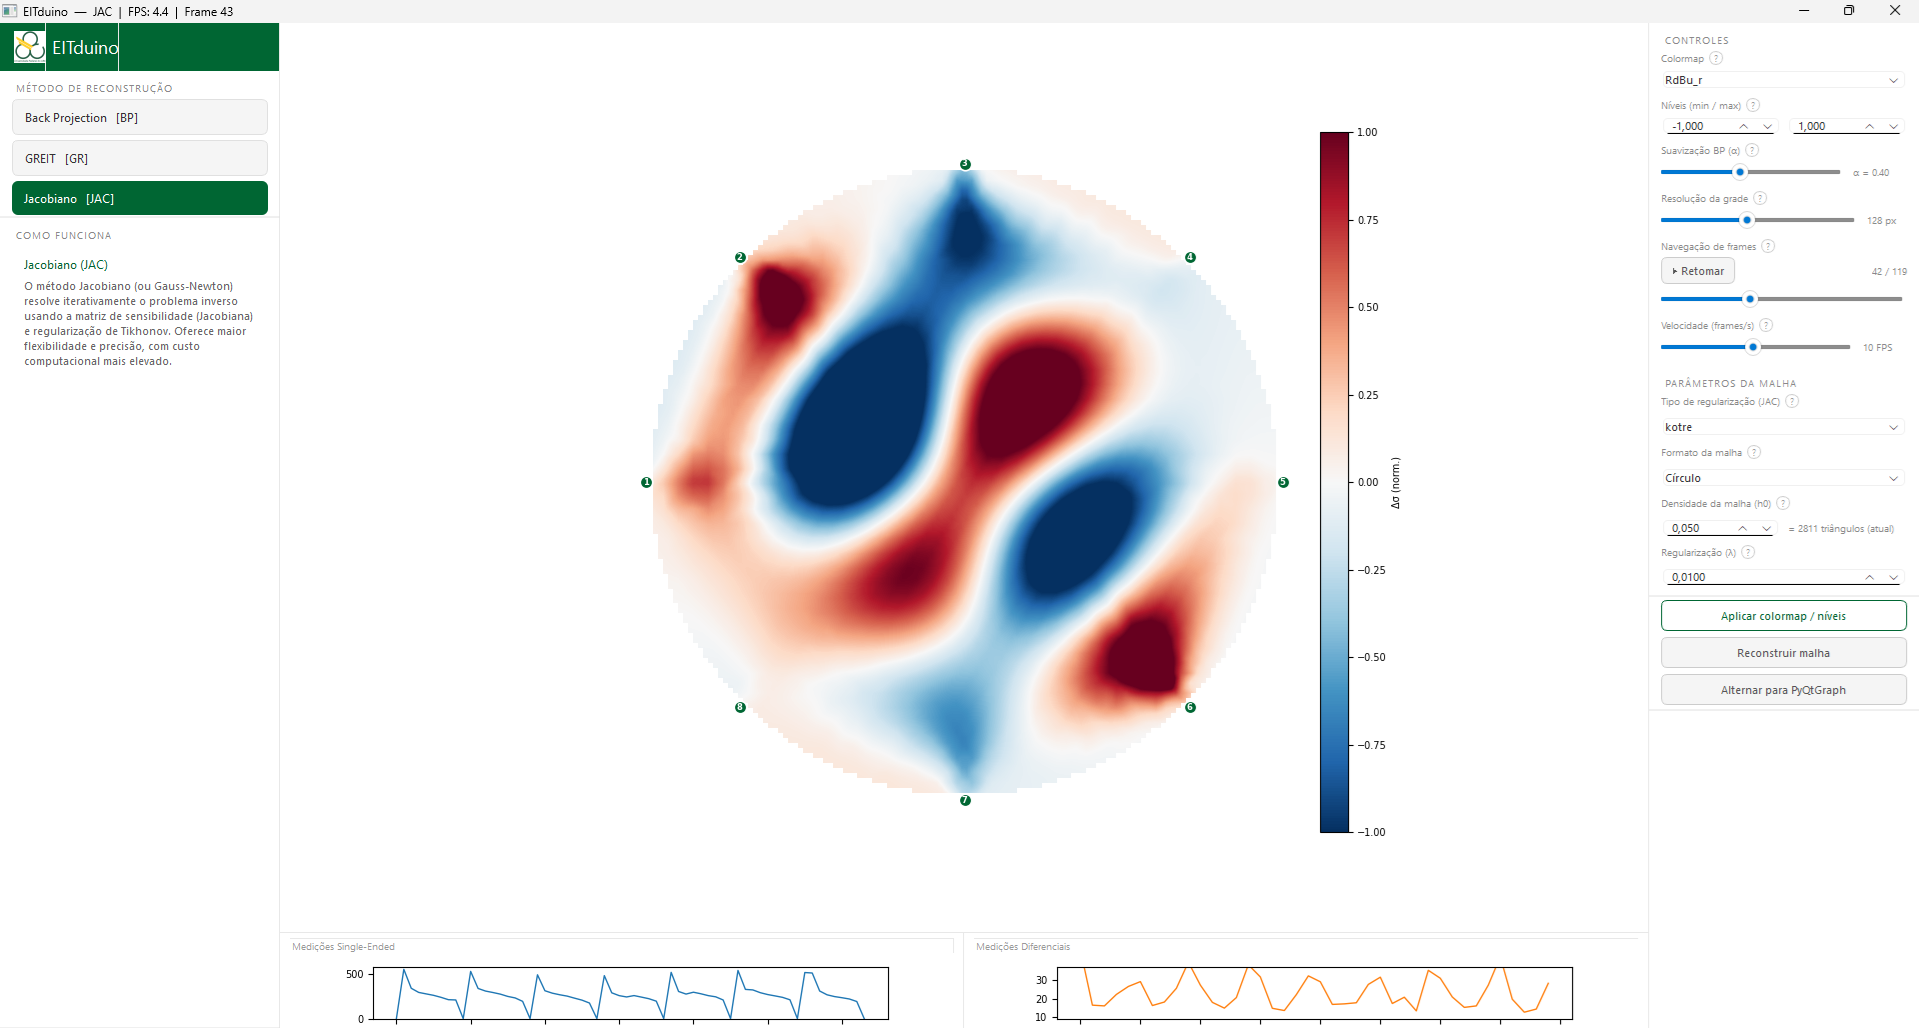
\includegraphics[width=0.85\textwidth]{pictures/JAC_Interface_Frame44_H0_05.png}
    \caption{Visão geral da interface principal com o método Back-Projection ativo (\textit{frame} 43, h0 = 0,10, α = 0,40).}
    \label{fig:interface_geral_bp}
\end{figure}

\section{Comparação entre métodos de reconstrução}
\label{sec:comparacao_metodos}

As figuras a seguir apresentam reconstruções obtidas com os métodos BP, JAC e GREIT em \textit{frame}s consecutivos do mesmo conjunto de dados experimentais. A comparação foi realizada a partir da mesma sequência de medições, mantendo os demais parâmetros de visualização constantes dentro de cada método, de modo a evidenciar diferenças relacionadas ao próprio algoritmo de reconstrução.

No método Back-Projection, mostrado na Figura~\ref{fig:bp_comparacao}, a região associada à haste pode ser identificada na porção superior-central do domínio, sobretudo pela presença de uma área azul mais intensa. Ainda assim, os contornos aparecem difusos e pouco definidos, o que dificulta a delimitação espacial mais precisa do objeto. Também se observam regiões avermelhadas na metade inferior da imagem sem correspondência física evidente com o arranjo experimental, caracterizando artefatos do processo de reconstrução. Entre os \textit{frame}s 43 e 44, a posição geral da região dominante se mantém, mas a imagem permanece espalhada e com baixo contraste local.

No método Jacobiano, apresentado nas Figuras~\ref{fig:jac_frame43} e \ref{fig:jac_frame44}, a posição da haste também é reconstruída na região superior-central do domínio, em concordância com o BP, mas com maior definição espacial e contraste mais localizado. No \textit{frame} 43, observa-se um padrão bipolar de alta intensidade, com alternância marcada entre regiões azuis e vermelhas. No \textit{frame} 44, a reconstrução assume uma forma visualmente mais limpa, com predomínio de uma região azul mais bem definida na área associada ao objeto. A comparação entre os dois \textit{frame}s mostra que o método foi capaz de preservar a localização da haste, mas também exibiu maior sensibilidade às variações entre \textit{frames} consecutivos, resultando em mudanças mais bruscas no padrão visual da reconstrução.

O método GREIT, ilustrado nas Figuras~\ref{fig:greit_frame43} e \ref{fig:greit_frame44}, produziu imagens visualmente mais suaves e estáveis entre \textit{frame}s consecutivos. A região de menor condutividade relativa permanece concentrada na parte superior-central do domínio, em posição compatível com a observada nos demais métodos, o que reforça a consistência qualitativa da localização da haste ao longo da reconstrução. Em contrapartida, o contraste é mais baixo e a transição espacial entre regiões é mais gradual, o que reduz a nitidez dos contornos. Também se destaca a presença de uma borda retangular visível na área reconstruída, decorrente da saída do método em grade regular de pixels. Em conjunto, os três algoritmos localizaram o objeto na mesma região do domínio, diferindo principalmente na definição dos contornos, no contraste e na estabilidade visual entre \textit{frame}s consecutivos.

\begin{figure}[H]
    \centering
    \begin{subfigure}[b]{0.48\textwidth}
        \centering
        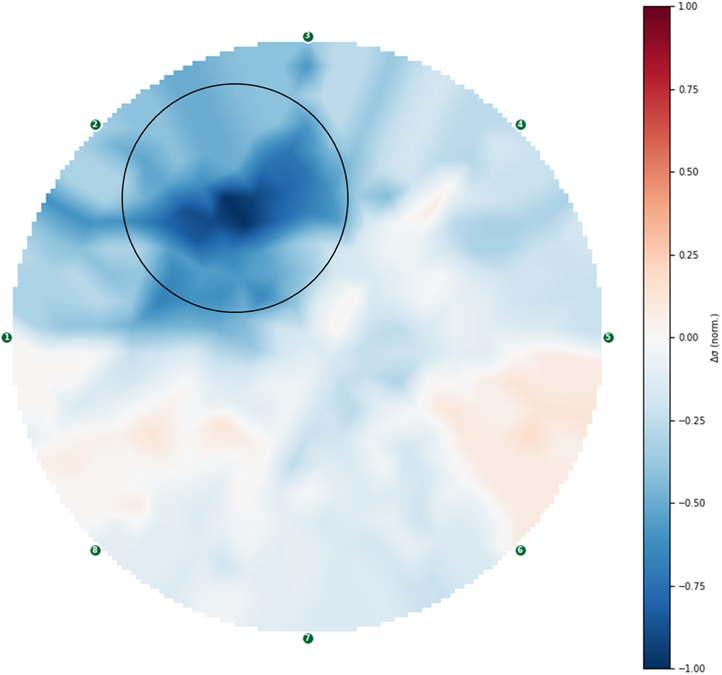
\includegraphics[width=\textwidth]{pictures/BP_Interface_Frame43.png}
        \caption{\textit{Frame} 43}
        \label{fig:bp_frame43}
    \end{subfigure}
    \hfill
    \begin{subfigure}[b]{0.48\textwidth}
        \centering
        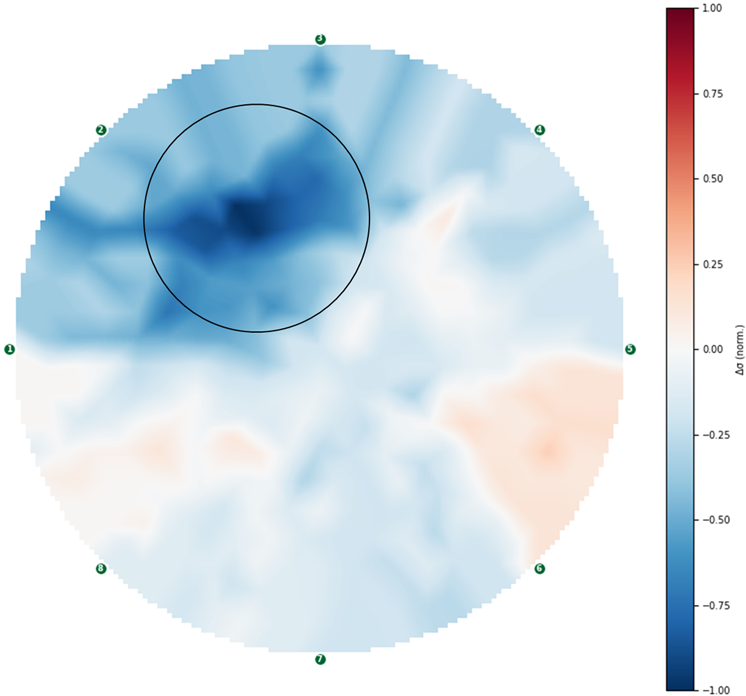
\includegraphics[width=\textwidth]{pictures/BP_Interface_Frame44.png}
        \caption{\textit{Frame} 44}
        \label{fig:bp_frame44}
    \end{subfigure}
    \caption{Reconstruções obtidas com o método Back-Projection (BP). Parâmetros: $h_0 = 0{,}10$, $\alpha = 0{,}40$, colormap \texttt{RdBu\_r}. O círculo indica a região de maior perturbação inferida, compatível com a presença do objeto.}
    \label{fig:bp_comparacao}
\end{figure}

\begin{figure}[H]
    \centering
    \begin{subfigure}[b]{0.48\textwidth}
        \centering
        
\includegraphics[width=\textwidth]{pictures/JAC_Interface_Frame43.png}
        \caption{\textit{Frame} 43}
        \label{fig:jac_frame43}
    \end{subfigure}
    \hfill
    \begin{subfigure}[b]{0.48\textwidth}
        \centering
        
\includegraphics[width=\textwidth]{pictures/JAC_Interface_Frame44.png}
        \caption{\textit{Frame} 44}
        \label{fig:jac_frame44}
    \end{subfigure}
    \caption{Reconstruções obtidas com o método Jacobiano (JAC). Parâmetros: \(h_0 = 0{,}10\), regularização \(\lambda = 0{,}0100\), método \texttt{kotre}, colormap \texttt{RdBu\_r}. O círculo indica a região de maior perturbação de condutividade inferida.}
    \label{fig:jac_comparacao}
\end{figure}

\begin{figure}[H]
    \centering
    \begin{subfigure}[b]{0.48\textwidth}
    \centering
    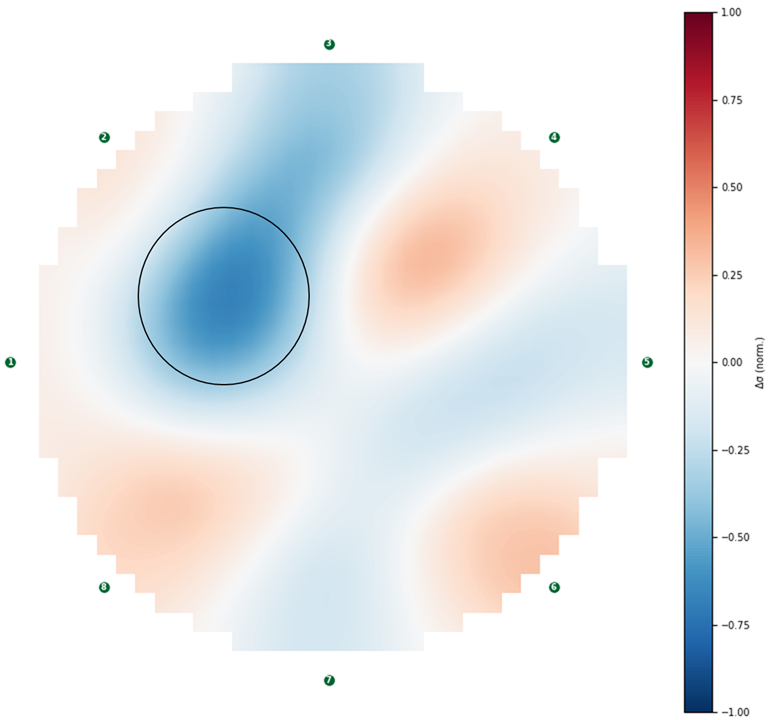
\includegraphics[width=\textwidth]{pictures/GREIT_Interface_Frame43.png}
    \caption{\textit{Frame} 43}
    \label{fig:greit_frame43}
    \end{subfigure}
    \hfill
    \begin{subfigure}[b]{0.48\textwidth}
        \centering
        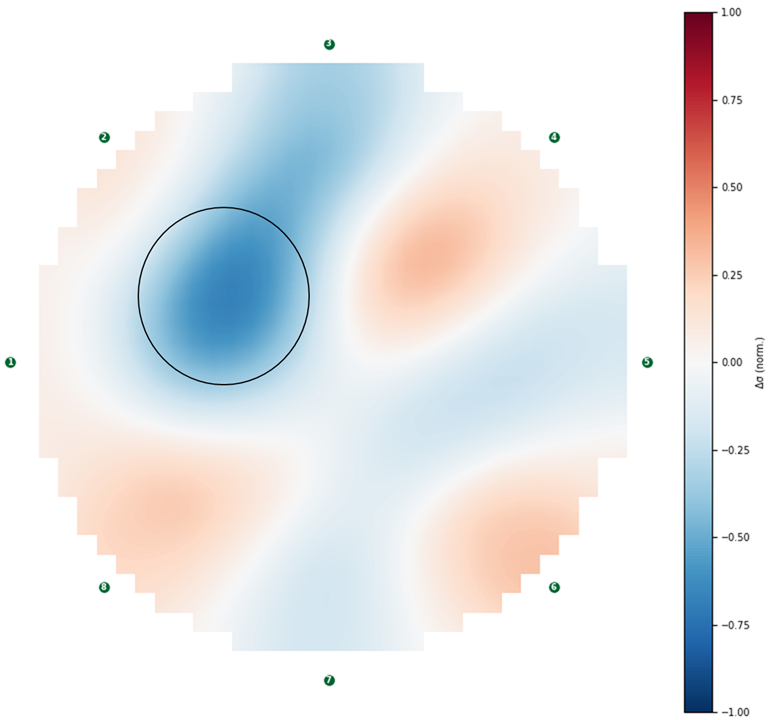
\includegraphics[width=\textwidth]{pictures/GREIT_Interface_Frame44.png}
        \caption{\textit{Frame} 44}
        \label{fig:greit_frame44}
    \end{subfigure}
    \caption{Reconstruções obtidas com o método GREIT. Parâmetros: \(h_0 = 0{,}10\), resolução da grade \(= 128\), colormap \texttt{RdBu\_r}. O círculo indica a região de maior perturbação de condutividade inferida.}
    \label{fig:greit_comparacao}
\end{figure}

\section{Efeito dos parâmetros configuráveis}
\label{sec:efeito_parametros}

\subsection{Densidade da malha (\(h_0\))}
\label{subsec:efeito_h0}

O parâmetro \(h_0\) define o comprimento máximo de aresta dos elementos triangulares da malha, expresso em unidades normalizadas em relação ao raio do domínio. Valores menores de \(h_0\) resultam em malhas mais refinadas, com maior número de elementos e resolução espacial mais alta, ao custo de maior custo computacional por quadro reconstruído.

As Figuras~\ref{fig:jac_h005} e \ref{fig:jac_h020} mostram o efeito da variação do parâmetro \(h_0\) na reconstrução obtida com o método Jacobiano. Na configuração mais refinada, com \(h_0 = 0{,}05\), a interface indica uma malha com 2811 triângulos, resultando em uma reconstrução visualmente mais detalhada, porém também mais fragmentada e com maior presença de artefatos locais. Na configuração mais grossa, com \(h_0 = 0{,}20\), a malha passa a conter 160 triângulos, produzindo uma imagem mais simples e suave, com menor nível de fragmentação. Essa comparação mostra que o refinamento da malha amplia a complexidade espacial da reconstrução, ao custo de maior carga computacional por quadro, dado o maior número de elementos envolvidos no cálculo.

\begin{figure}[htbp]
    \centering
    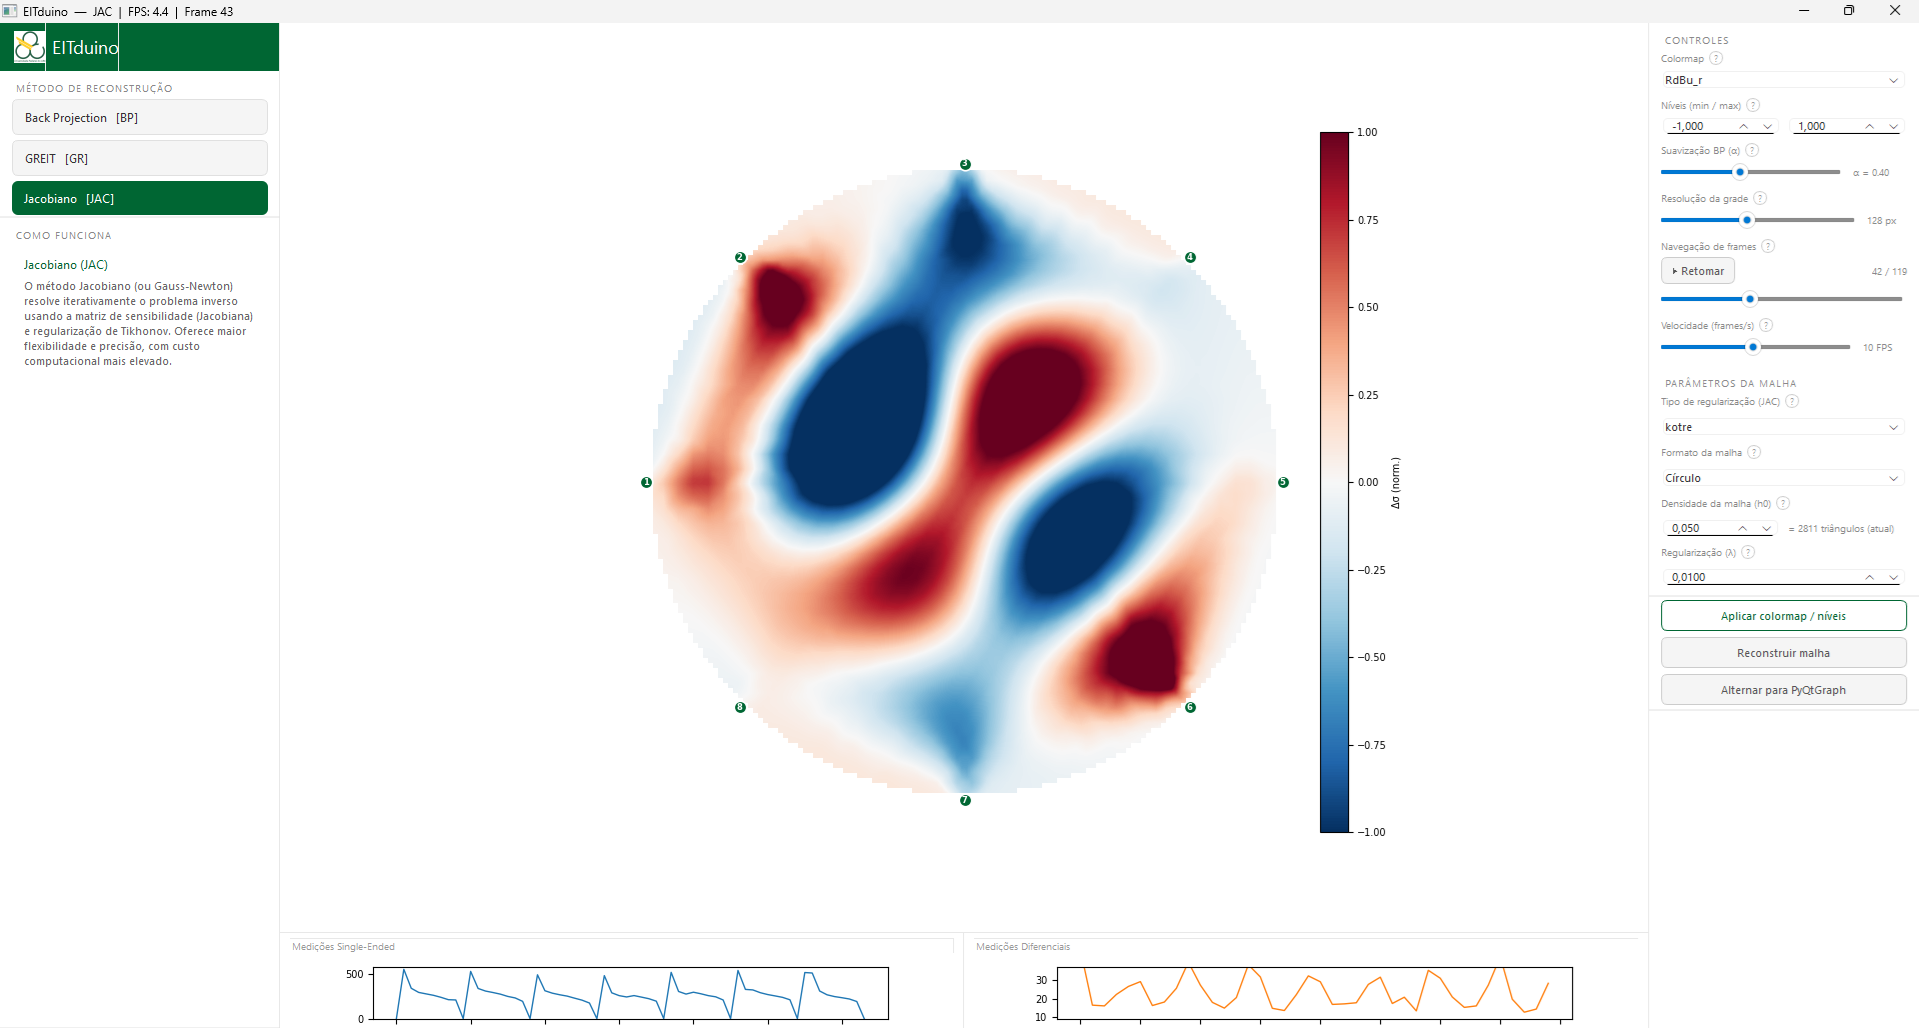
\includegraphics[width=0.85\textwidth]{pictures/JAC_Interface_Frame44_H0_05.png}
    \caption{Reconstrução obtida com o método Jacobiano no \textit{frame} 44, utilizando \(h_0 = 0{,}05\). A interface indica uma malha com 2811 triângulos.}
    \label{fig:jac_h005}
\end{figure}

\begin{figure}[htbp]
    \centering
    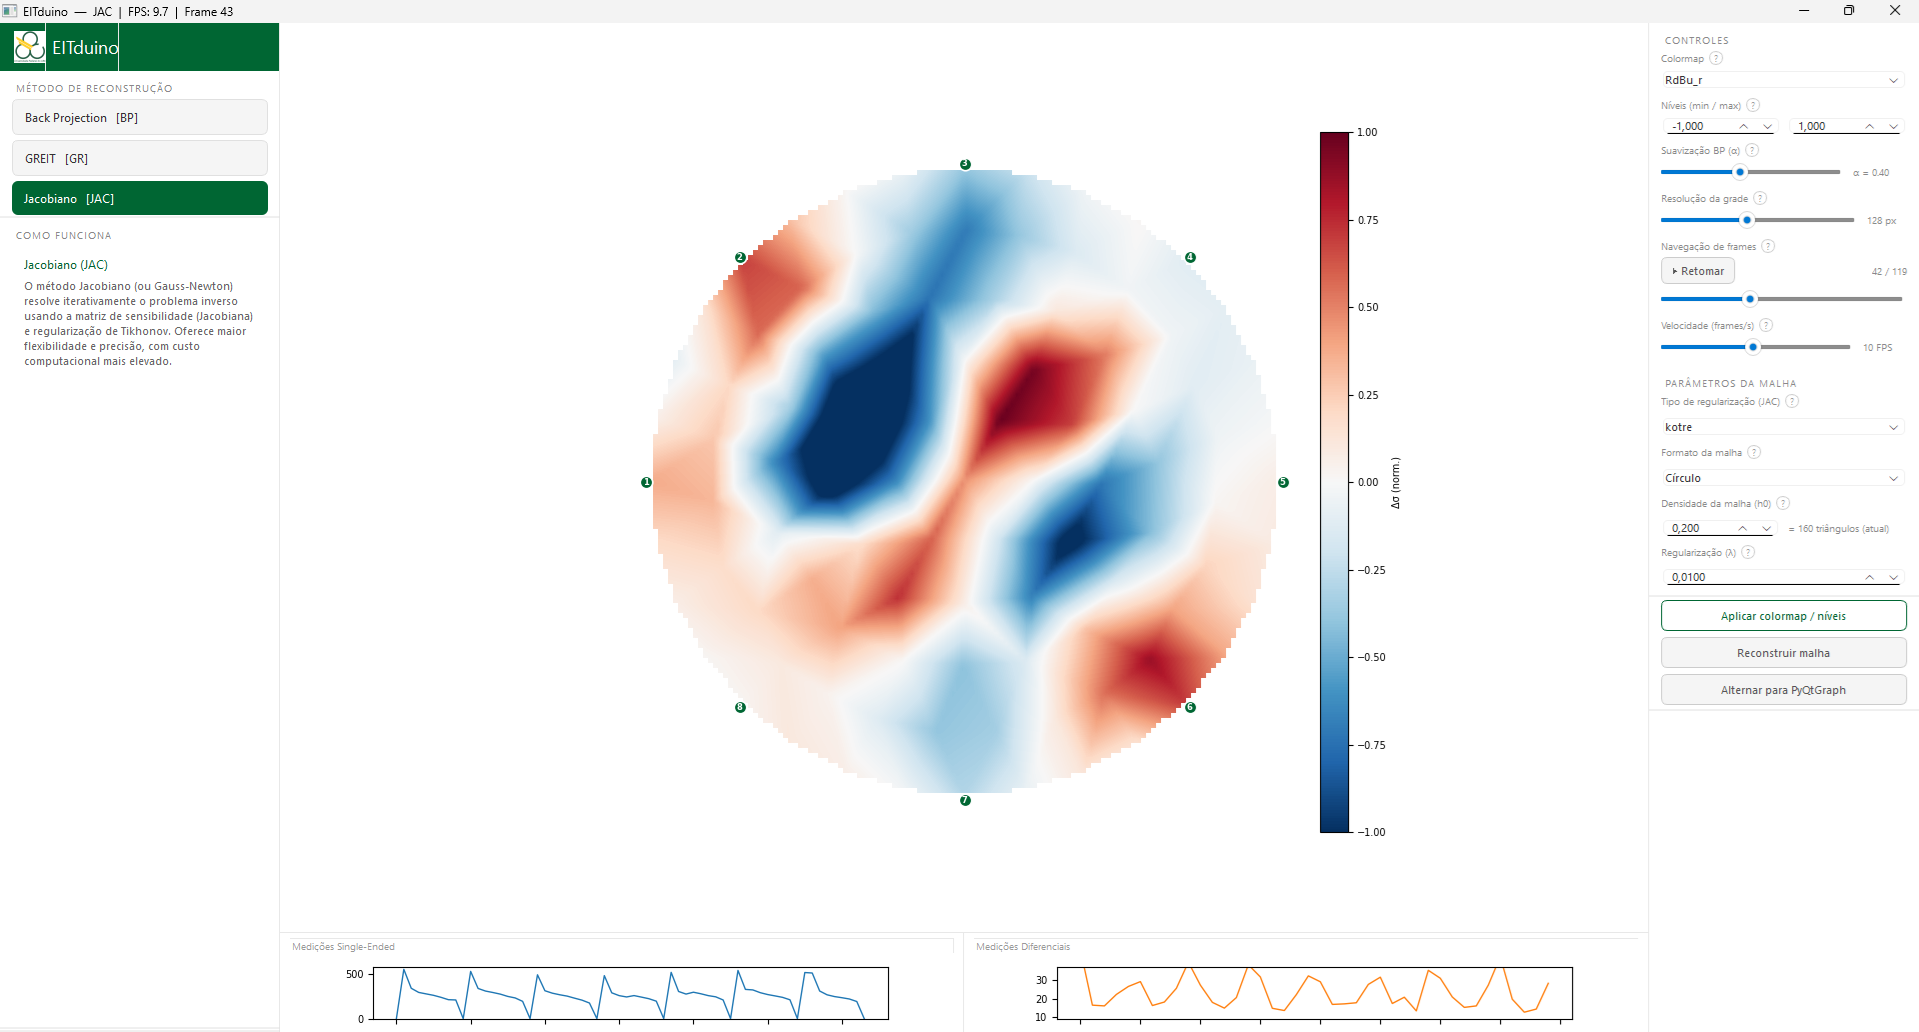
\includegraphics[width=0.85\textwidth]{pictures/JAC_Interface_Frame44_H0_2.png}
    \caption{Reconstrução obtida com o método Jacobiano no \textit{frame} 44, utilizando \(h_0 = 0{,}20\). A interface indica uma malha com 160 triângulos.}
    \label{fig:jac_h020}
\end{figure}

\subsection{Suavização temporal (\(\alpha\))}
\label{subsec:efeito_alpha}

O parâmetro \(\alpha \in [0, 1]\) é adimensional e controla o peso atribuído à reconstrução do quadro anterior na composição da imagem exibida, conforme definido na Equação~\ref{eq:suavizacao_temporal}.

As Figuras~\ref{fig:bp_alpha01} e \ref{fig:bp_alpha09} ilustram o efeito do parâmetro de suavização temporal \(\alpha\) nas reconstruções obtidas com o método Back-Projection. Com \(\alpha = 0{,}10\), a imagem responde mais diretamente ao \textit{frame} corrente, preservando com maior fidelidade as variações instantâneas, mas também exibindo maior oscilação visual. Com \(\alpha = 0{,}90\), a reconstrução passa a variar de forma mais gradual entre \textit{frames}, produzindo um resultado visualmente mais estável. A comparação entre essas duas configurações mostra que o aumento de \(\alpha\) reduz a cintilação entre \textit{frames} consecutivos, embora também introduza um leve fator de inércia na resposta visual do método. Como o efeito da suavização temporal se manifesta principalmente na transição entre quadros consecutivos, sua influência é mais evidente durante a reprodução animada dos dados do que na comparação entre imagens estáticas.

\begin{figure}[htbp]
    \centering
    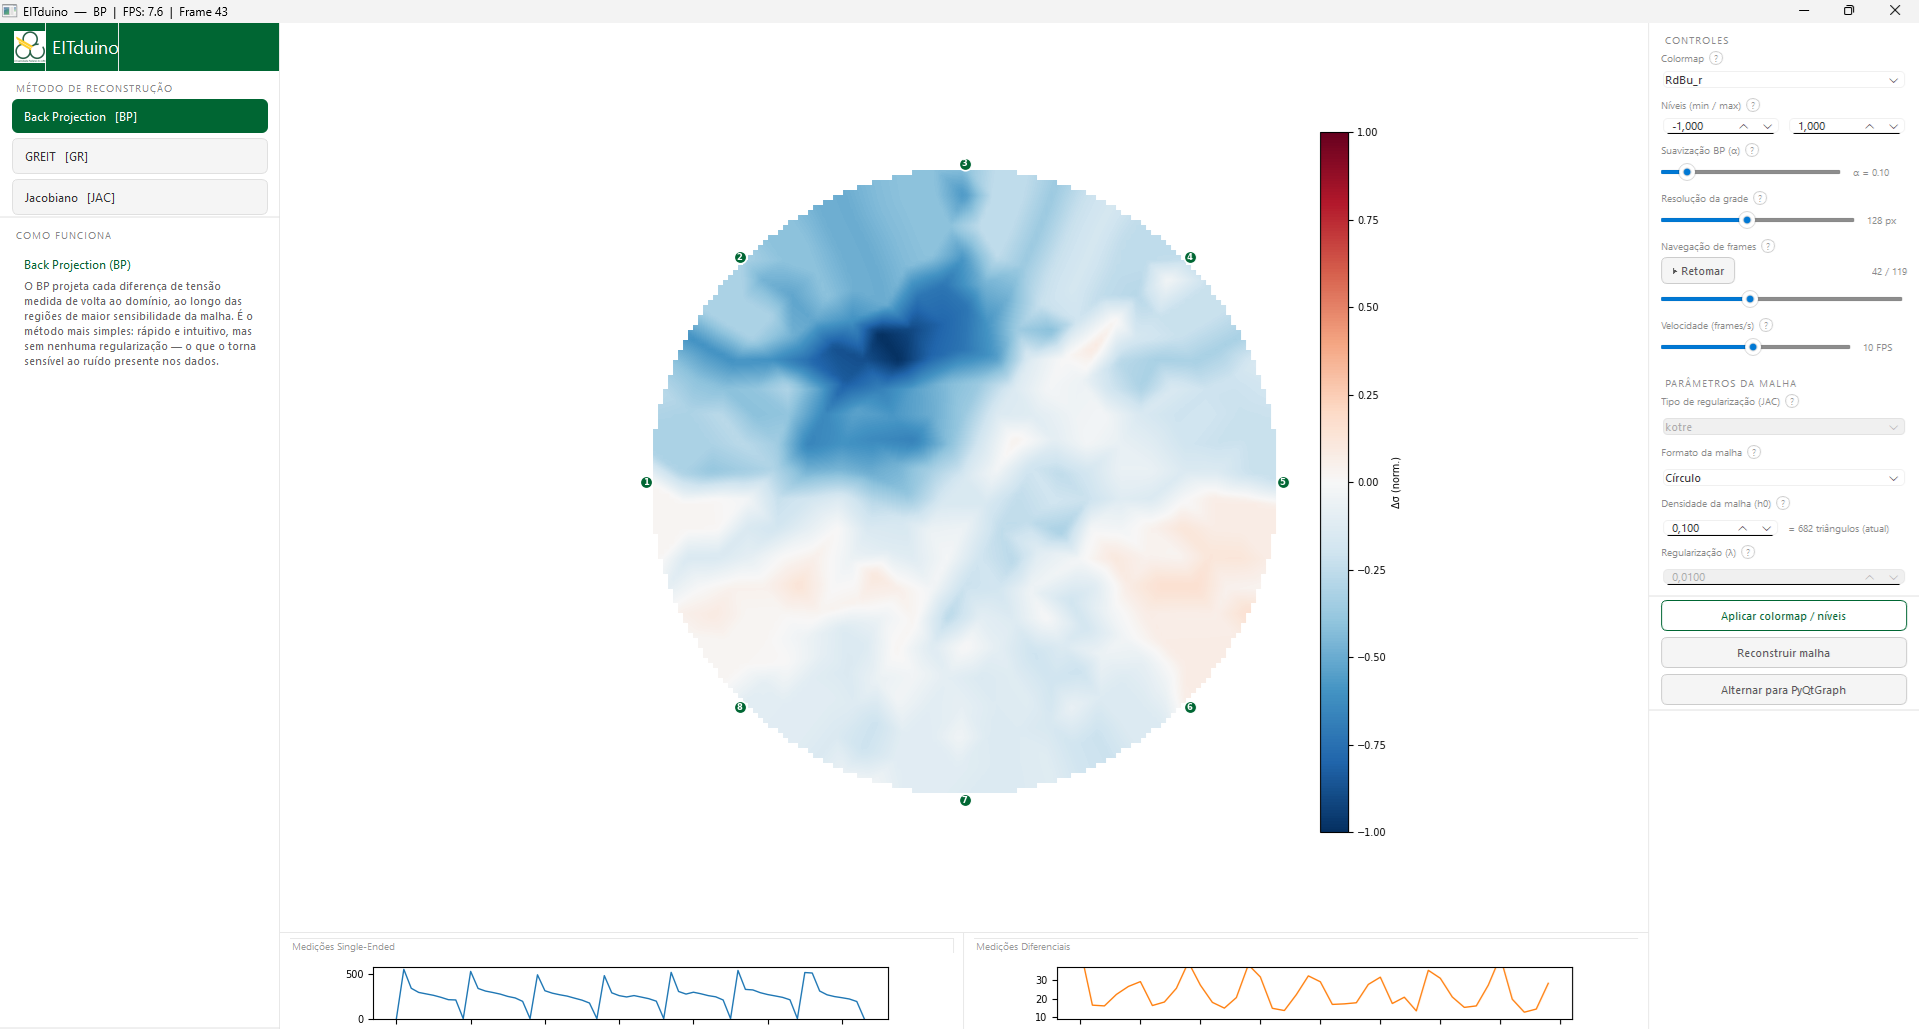
\includegraphics[width=0.85\textwidth]{pictures/BP_Interface_Frame43_alpha0_1.png}
    \caption{Reconstrução obtida com o método Back-Projection no \textit{frame} 43, utilizando \(\alpha = 0{,}10\).}
    \label{fig:bp_alpha01}
\end{figure}

\begin{figure}[htbp]
    \centering
    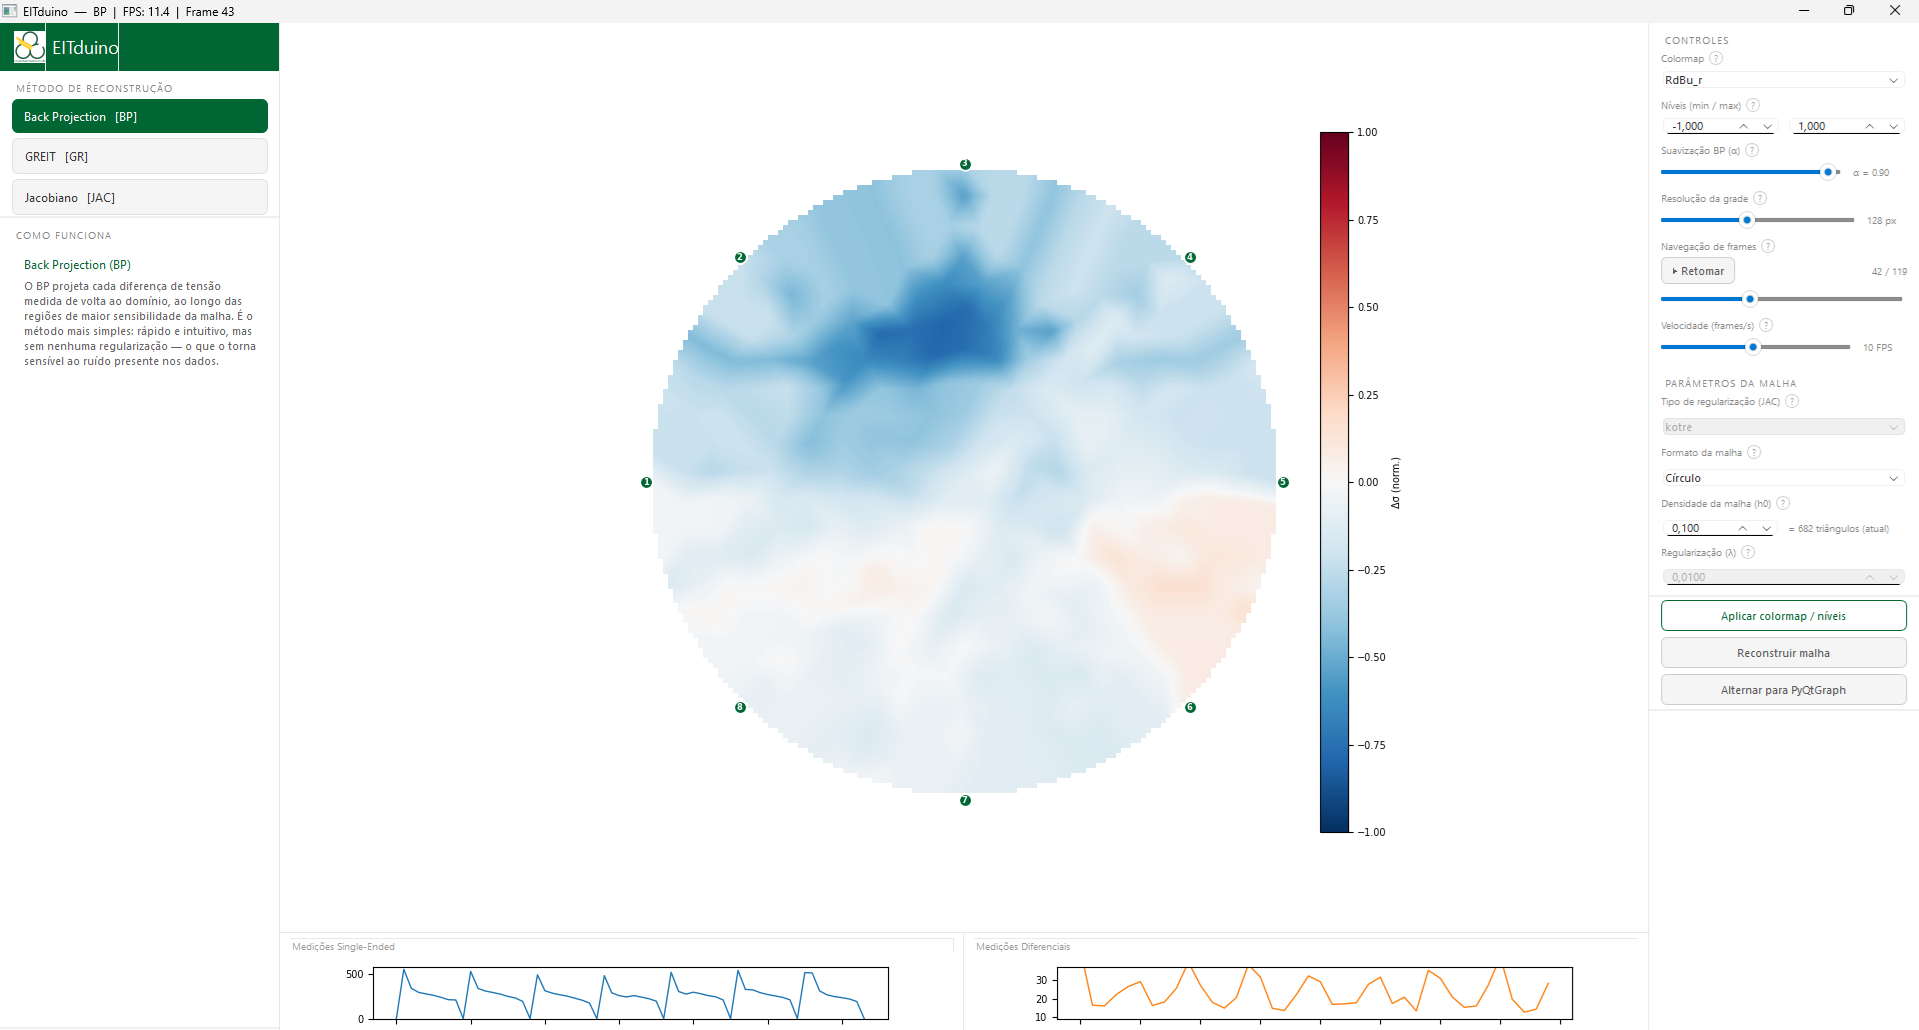
\includegraphics[width=0.85\textwidth]{pictures/BP_Interface_Frame43_alpha0_9.png}
    \caption{Reconstrução obtida com o método Back-Projection no \textit{frame} 43, utilizando \(\alpha = 0{,}90\).}
    \label{fig:bp_alpha09}
\end{figure}

\subsection{Efeito da regularização (\(\lambda\))}
\label{subsec:efeito_regularizacao}

As Figuras~\ref{fig:jac_reg_0001} a \ref{fig:greit_reg_1} mostram o efeito da variação do parâmetro de regularização \(\lambda\) nas reconstruções obtidas com os métodos Jacobiano e GREIT. Para essa comparação, foi utilizado o mesmo \textit{frame} do conjunto experimental, mantendo-se constantes a geometria da malha, o valor de \(h_0\), a resolução da grade e os demais parâmetros de visualização. Foram testados quatro valores de regularização em cada método: \(\lambda = 0{,}0001\), \(\lambda = 0{,}01\), \(\lambda = 0{,}1\) e \(\lambda = 1{,}0\).

No caso do método Jacobiano, a progressão entre as Figuras~\ref{fig:jac_reg_0001}, \ref{fig:jac_reg_001}, \ref{fig:jac_reg_01} e \ref{fig:jac_reg_1} evidencia de forma clara o efeito da regularização sobre a reconstrução. Com \(\lambda = 0{,}0001\), a imagem apresenta alto contraste, contornos mais agudos e forte presença de artefatos bipolares, indicando predominância da aderência aos dados medidos sobre a suavização da solução. Com \(\lambda = 0{,}01\), o padrão visual permanece semelhante, mas ligeiramente mais contido. Em \(\lambda = 0{,}1\), a reconstrução torna-se visivelmente mais suave, com redução dos artefatos mais intensos e uma localização mais legível da região associada à haste. Já com \(\lambda = 1{,}0\), a imagem fica amplamente atenuada, restando apenas uma região azul difusa e de baixo contraste, o que indica predominância da regularização sobre a contribuição dos dados experimentais.

No método GREIT, observa-se comportamento análogo, embora com o padrão espacial característico do próprio algoritmo. Nas Figuras~\ref{fig:greit_reg_0001} e \ref{fig:greit_reg_001}, a reconstrução exibe regiões azul-vermelho bem definidas e com maior contraste, ainda com forte influência do termo de dados. Na Figura~\ref{fig:greit_reg_01}, o padrão torna-se mais suave e menos intenso, com transições espaciais mais graduais. Na Figura~\ref{fig:greit_reg_1}, a imagem aparece quase completamente suprimida, permanecendo apenas uma variação residual de baixa intensidade. Em ambos os métodos, a transição entre imagens mais nítidas e mais ruidosas para imagens mais suaves e mais atenuadas torna visível, na própria interface, o compromisso entre fidelidade aos dados e estabilidade da solução.

Esse comportamento está de acordo com a formulação teórica apresentada para o problema inverso regularizado: a escolha de \(\lambda\) controla diretamente o equilíbrio entre aderência às medições e suavização da reconstrução, efeito que pode ser observado qualitativamente de forma imediata na interface desenvolvida.

\begin{figure}[htbp]
    \centering
    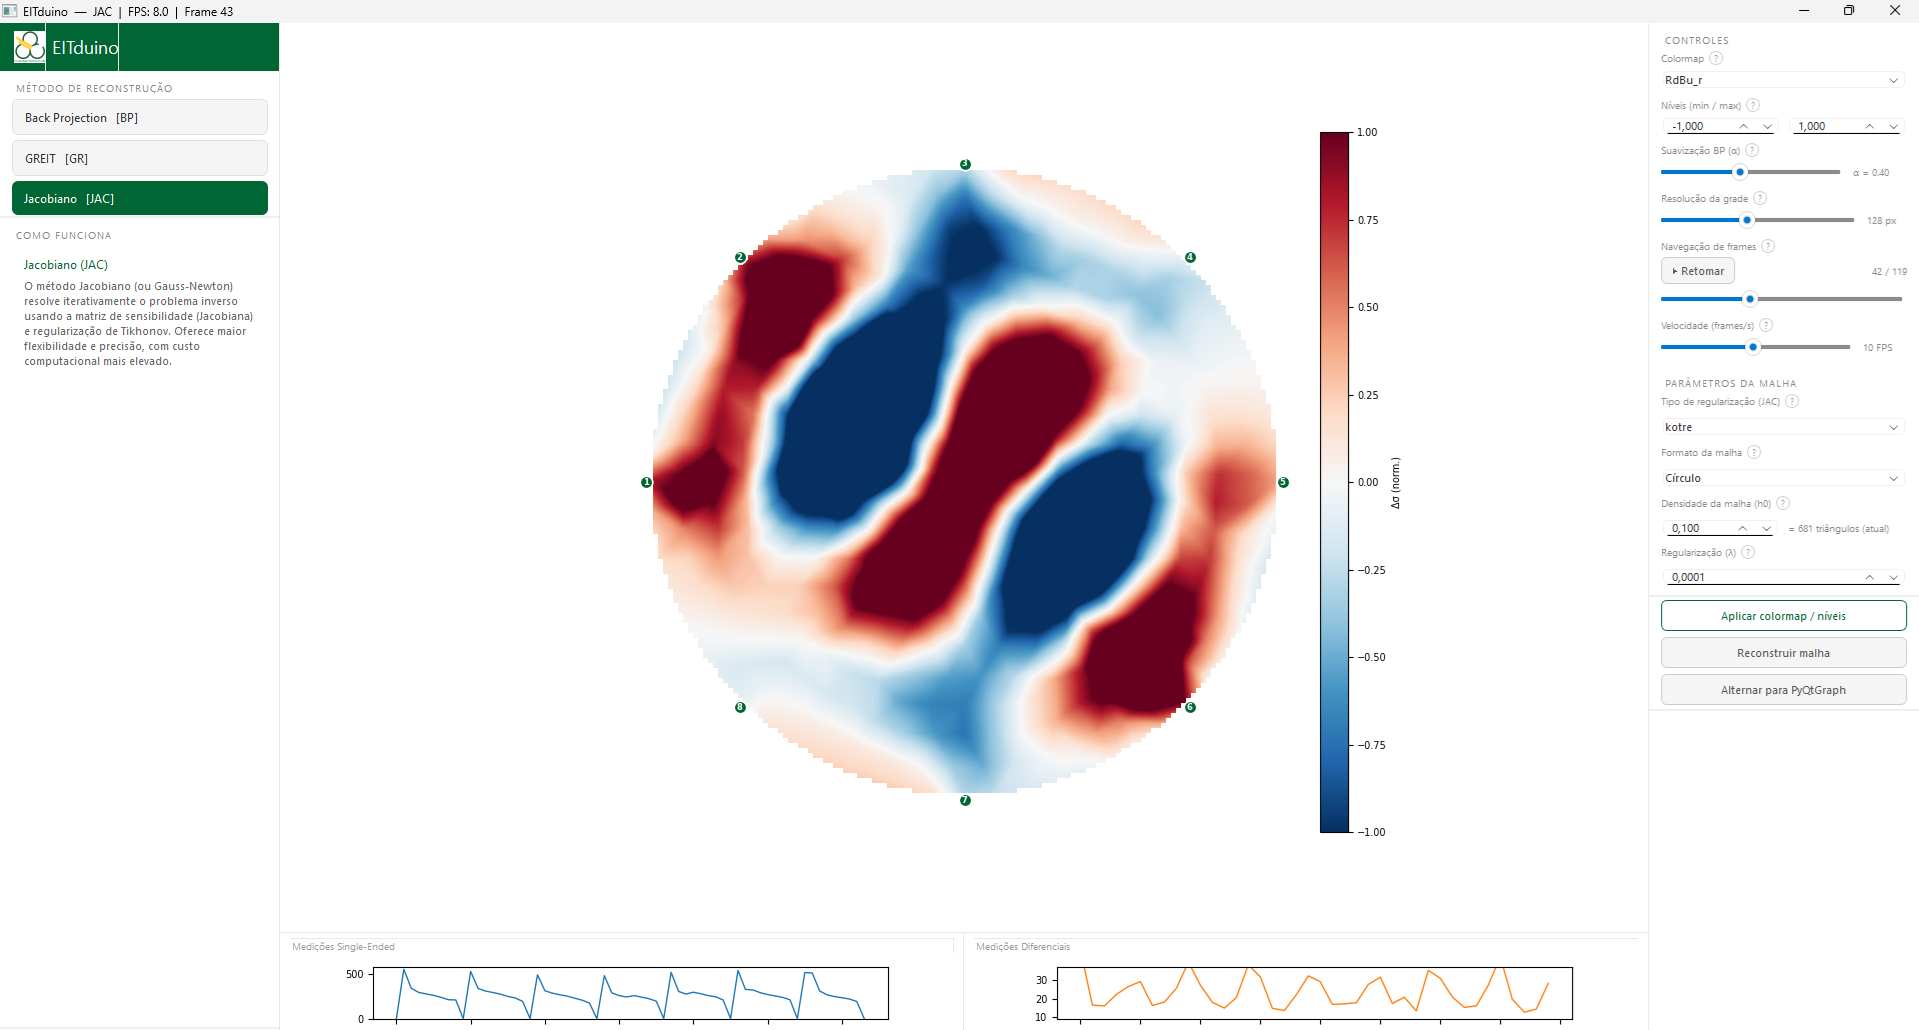
\includegraphics[width=0.85\textwidth]{pictures/JAC_pyQT_Reg0_0001.png}
    \caption{Reconstrução obtida com o método Jacobiano no \textit{frame} 43, utilizando \(\lambda = 0{,}0001\).}
    \label{fig:jac_reg_0001}
\end{figure}

\begin{figure}[htbp]
    \centering
    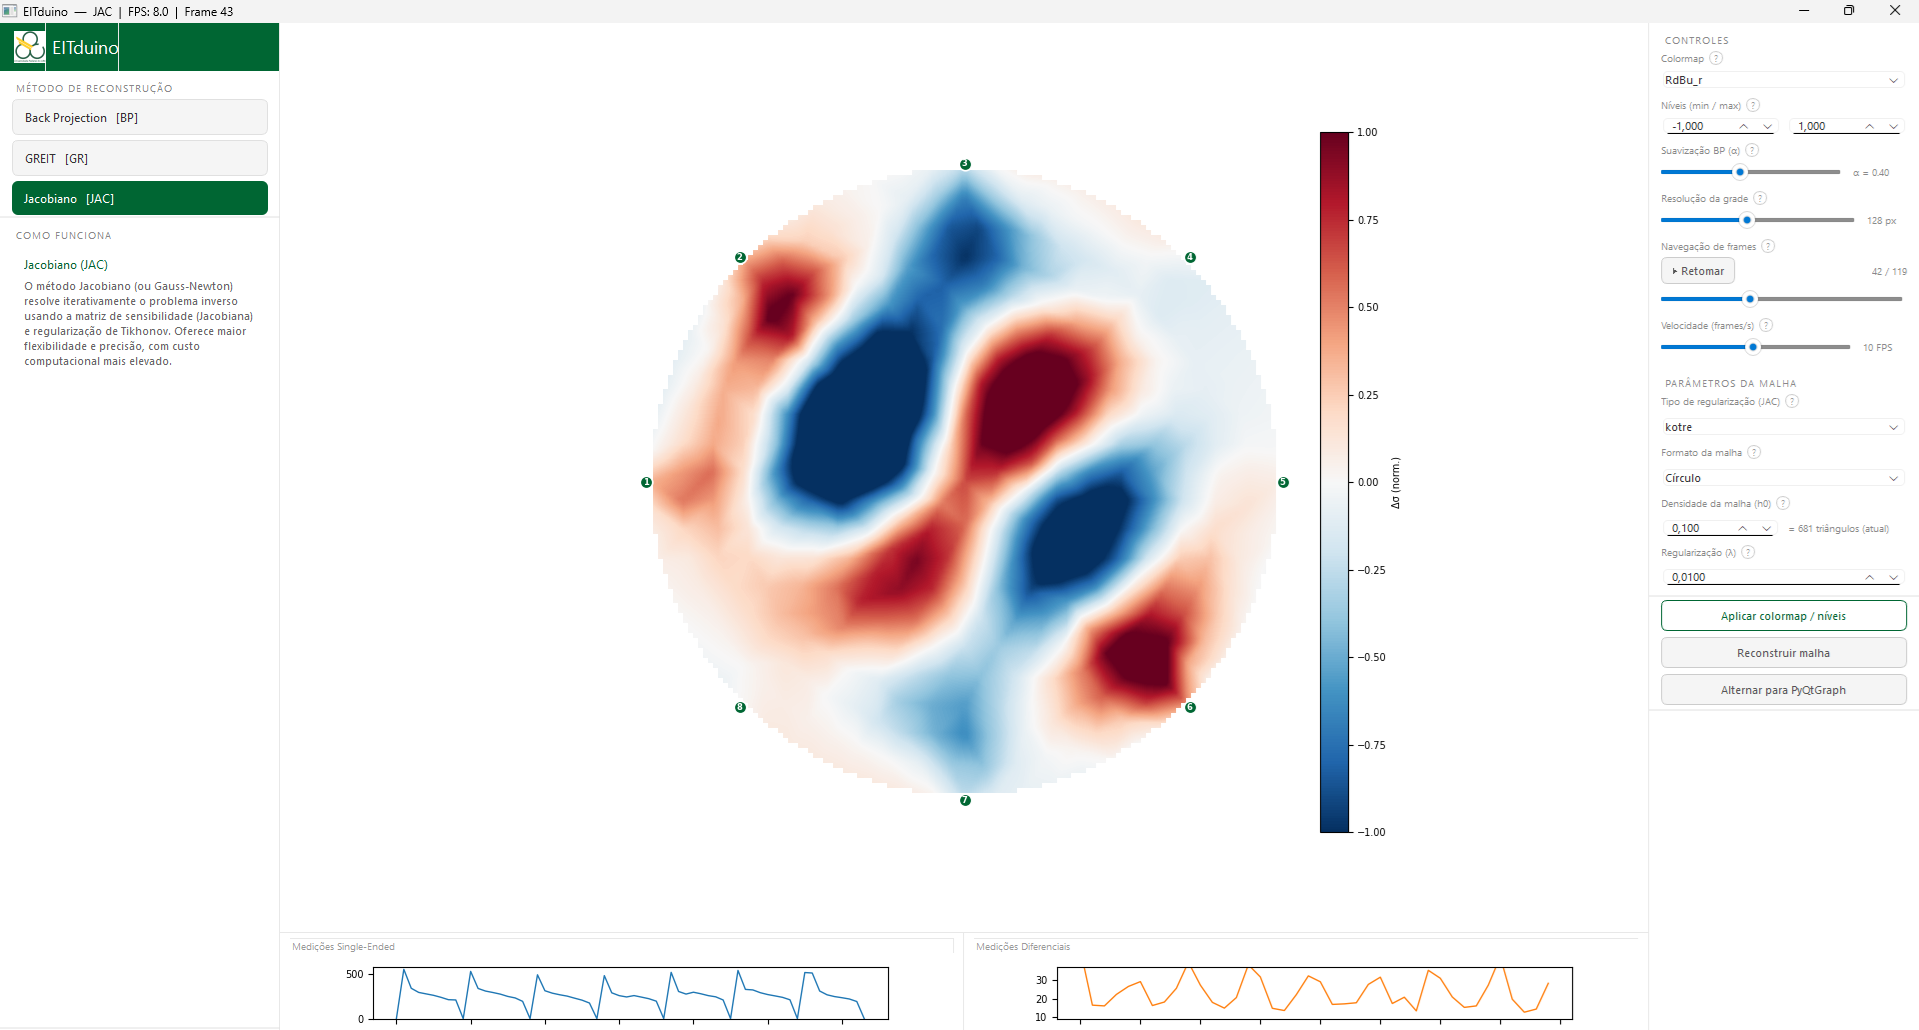
\includegraphics[width=0.85\textwidth]{pictures/JAC_pyQT_Reg0_01.png}
    \caption{Reconstrução obtida com o método Jacobiano no \textit{frame} 43, utilizando \(\lambda = 0{,}01\).}
    \label{fig:jac_reg_001}
\end{figure}

\begin{figure}[htbp]
    \centering
    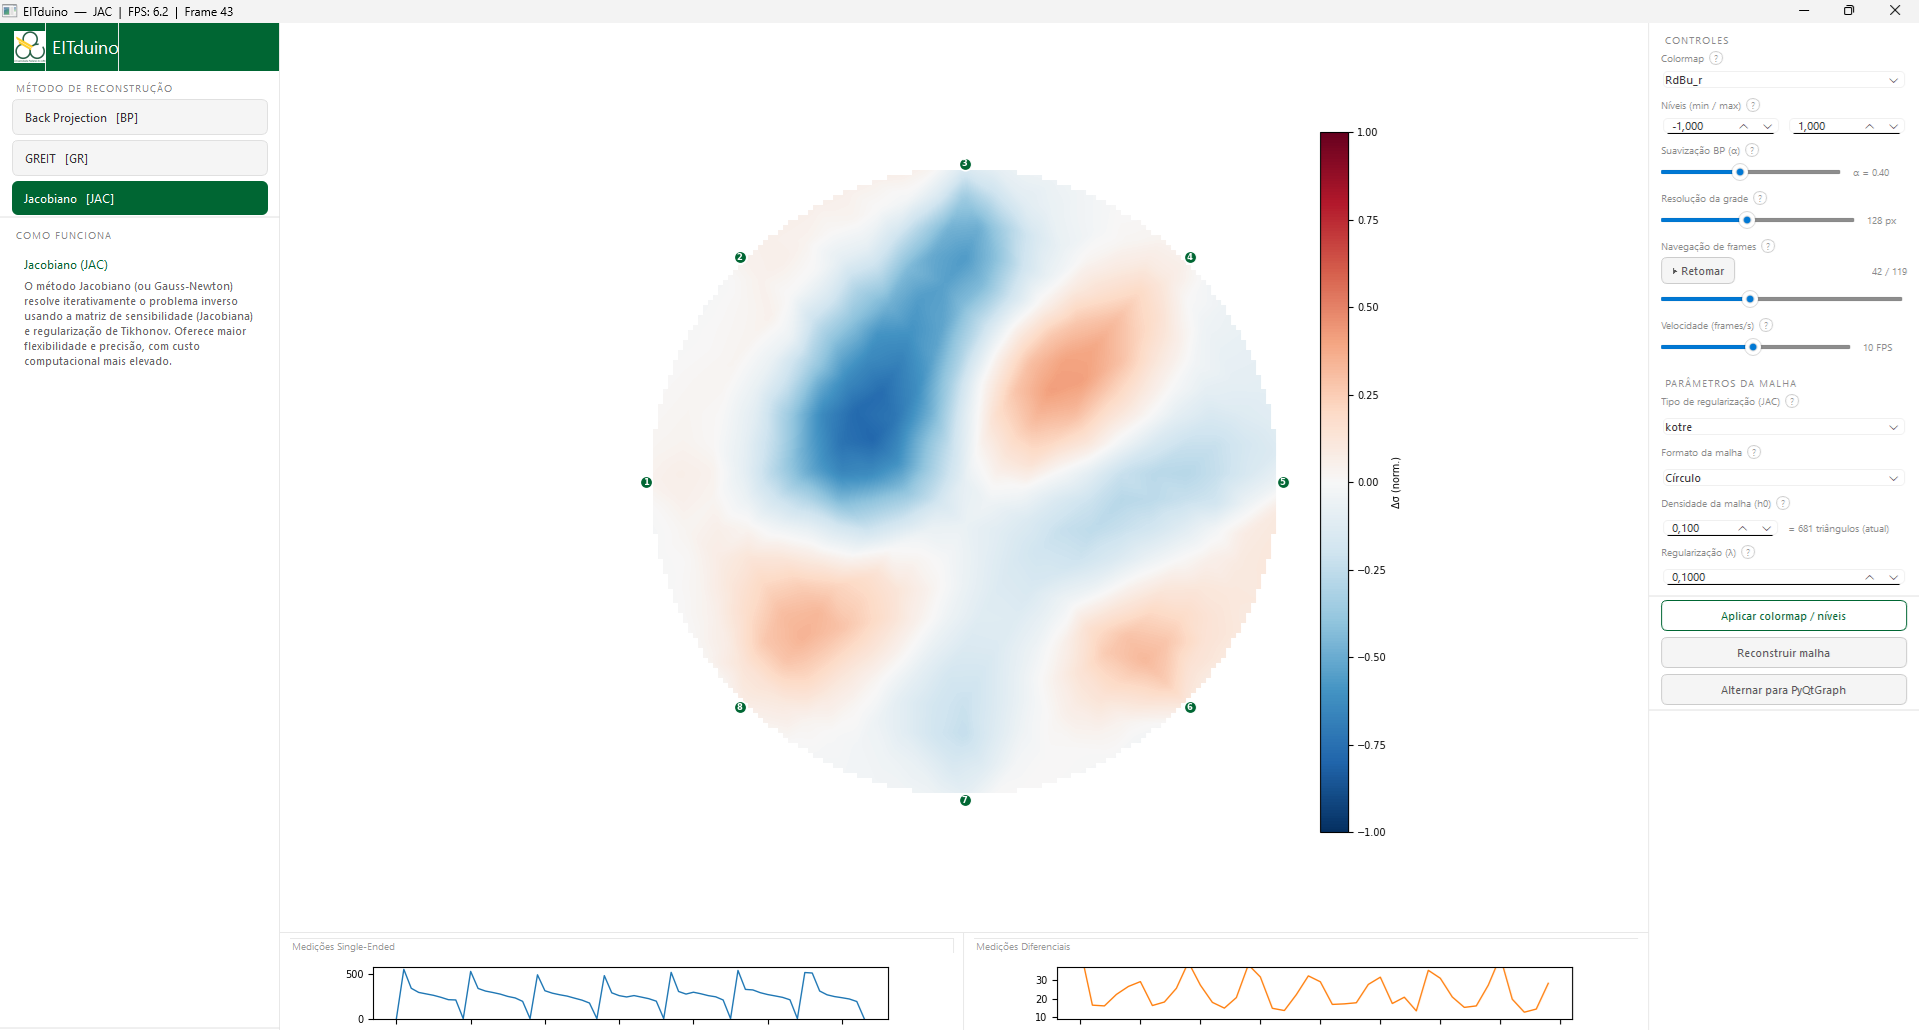
\includegraphics[width=0.85\textwidth]{pictures/JAC_pyQT_Reg0_1.png}
    \caption{Reconstrução obtida com o método Jacobiano no \textit{frame} 43, utilizando \(\lambda = 0{,}1\).}
    \label{fig:jac_reg_01}
\end{figure}

\begin{figure}[htbp]
    \centering
    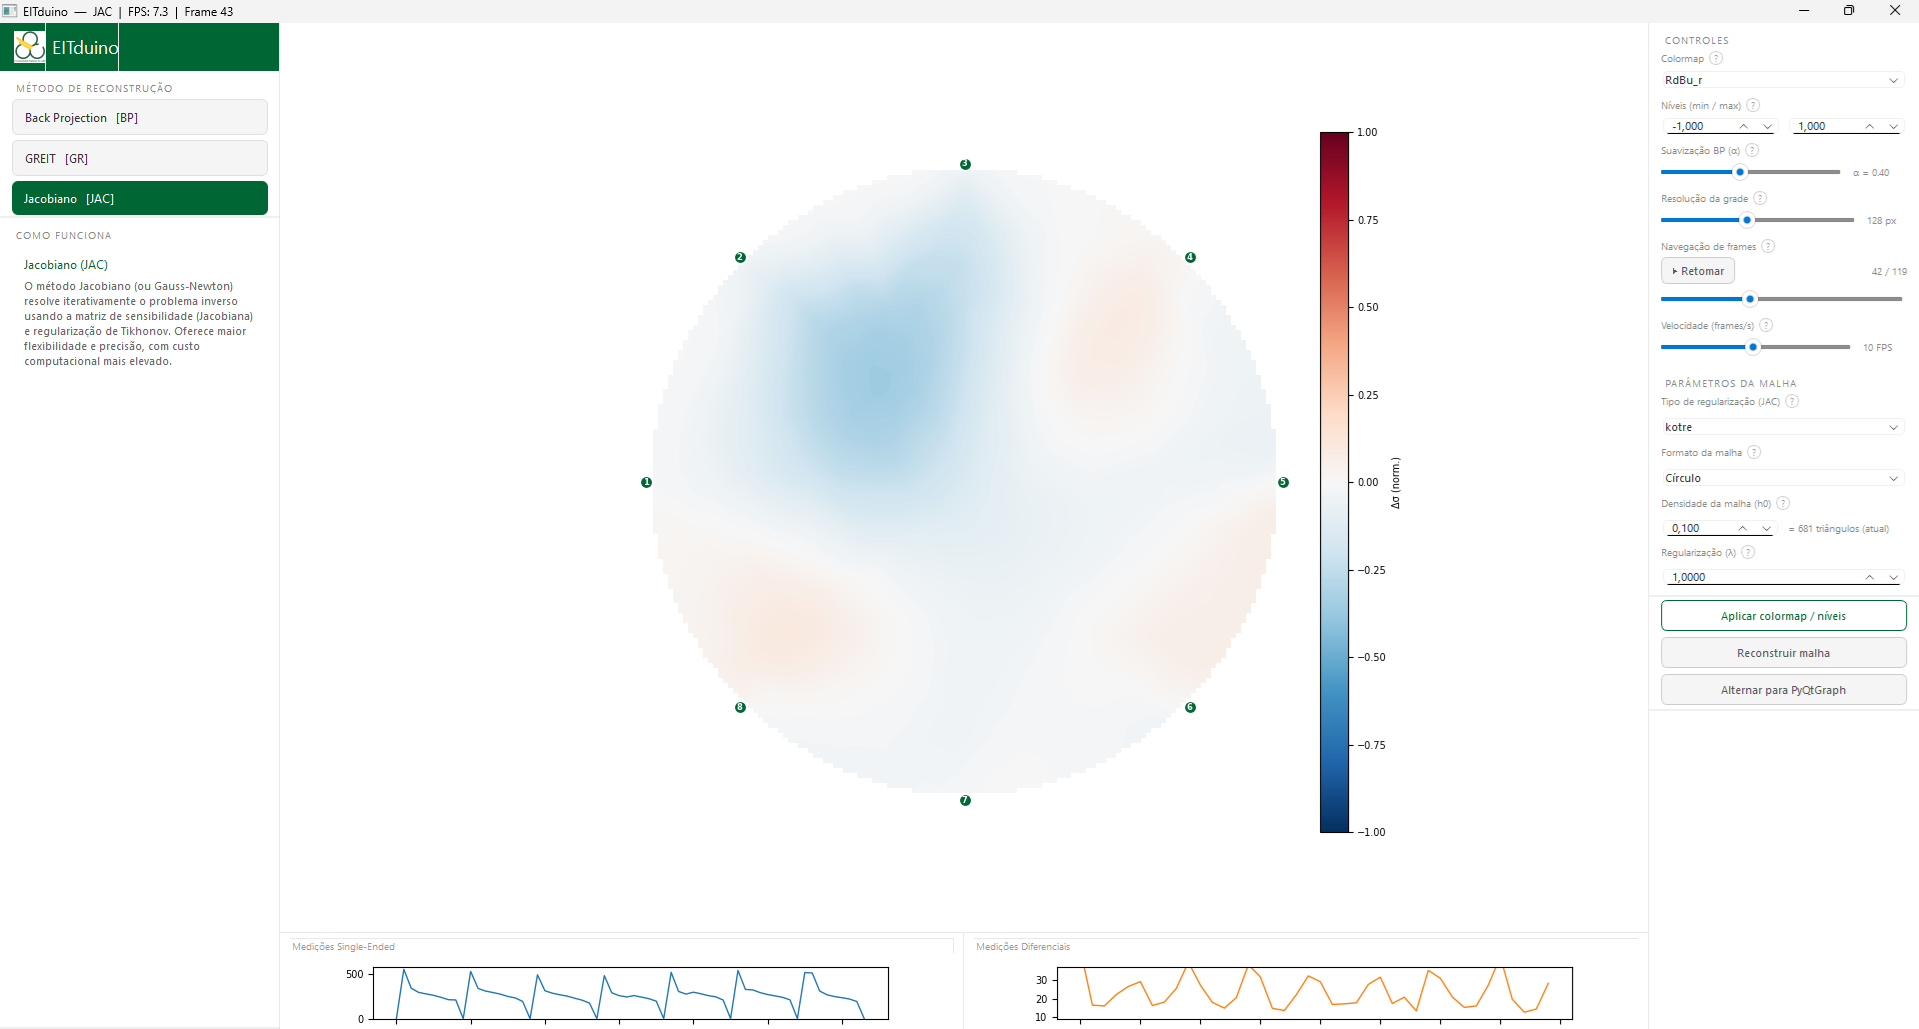
\includegraphics[width=0.85\textwidth]{pictures/JAC_pyQT_Reg1.png}
    \caption{Reconstrução obtida com o método Jacobiano no \textit{frame} 43, utilizando \(\lambda = 1{,}0\).}
    \label{fig:jac_reg_1}
\end{figure}

\begin{figure}[htbp]
    \centering
    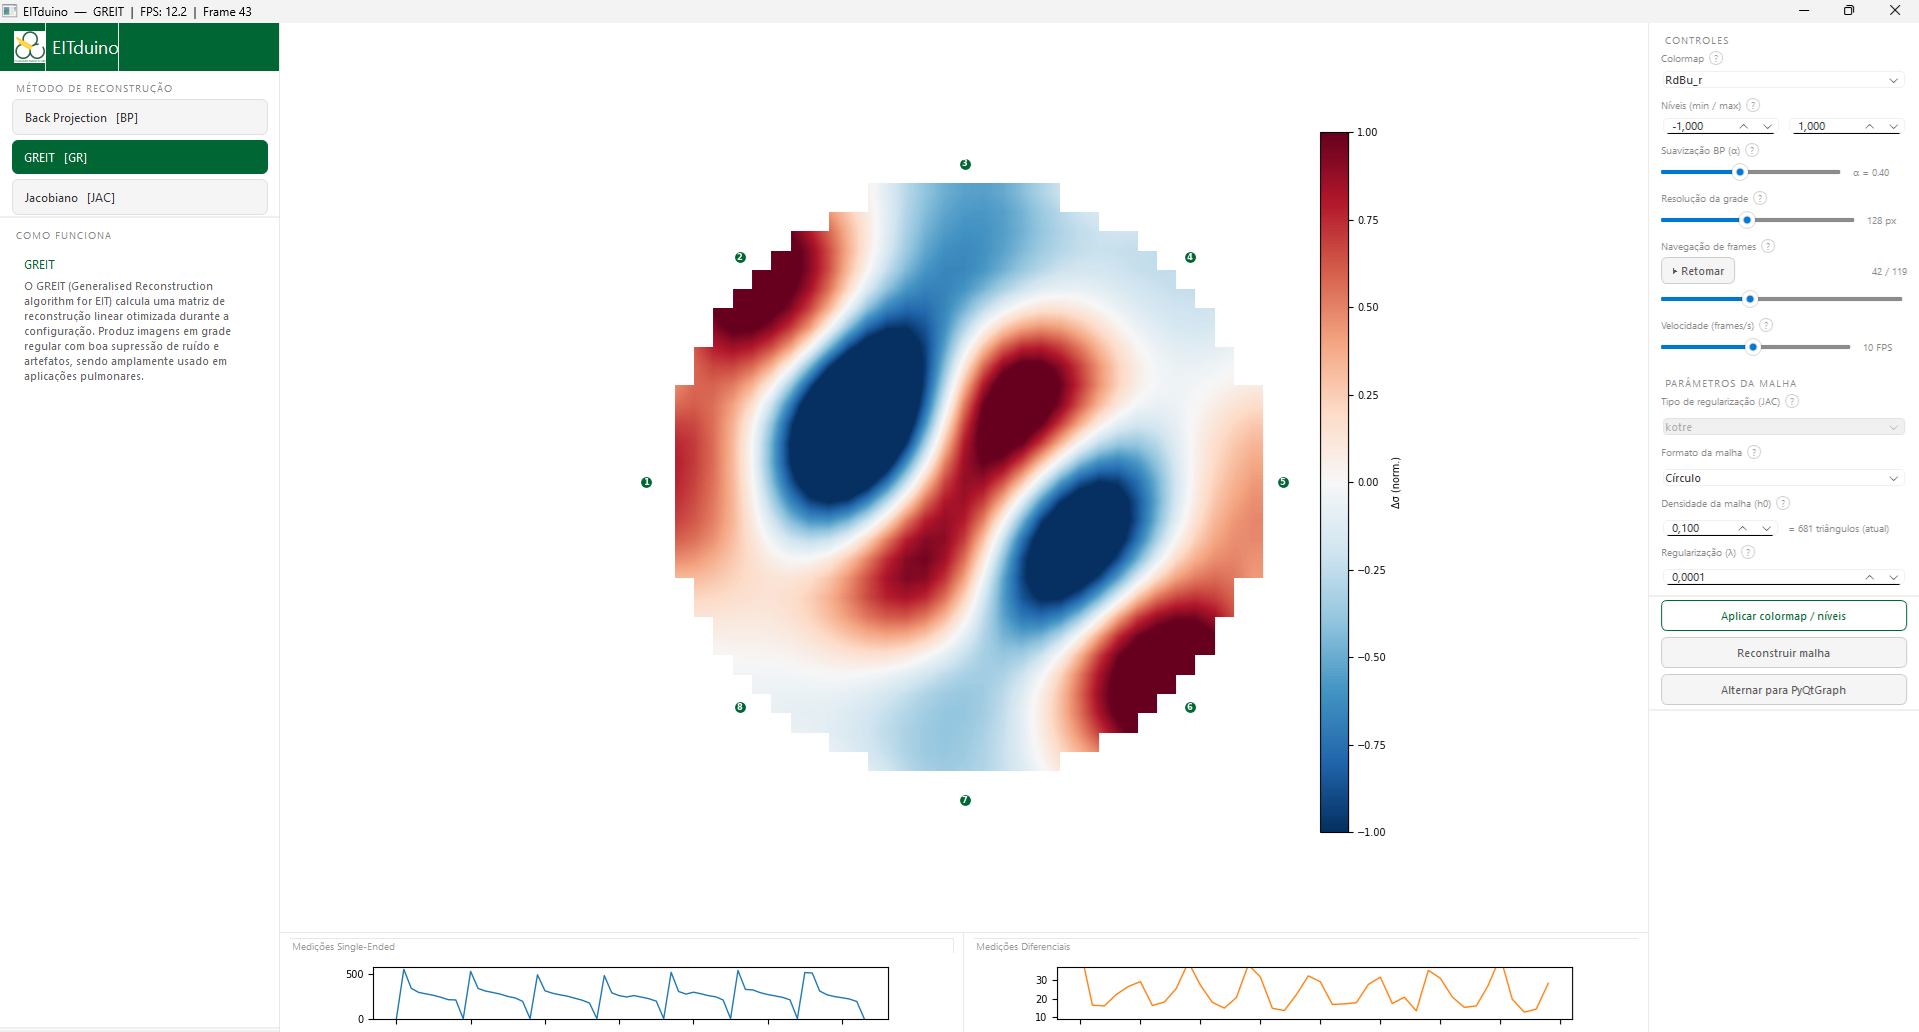
\includegraphics[width=0.85\textwidth]{pictures/GREIT_pyQT_Reg0_0001.png}
    \caption{Reconstrução obtida com o método GREIT no \textit{frame} 43, utilizando \(\lambda = 0{,}0001\).}
    \label{fig:greit_reg_0001}
\end{figure}

\begin{figure}[htbp]
    \centering
    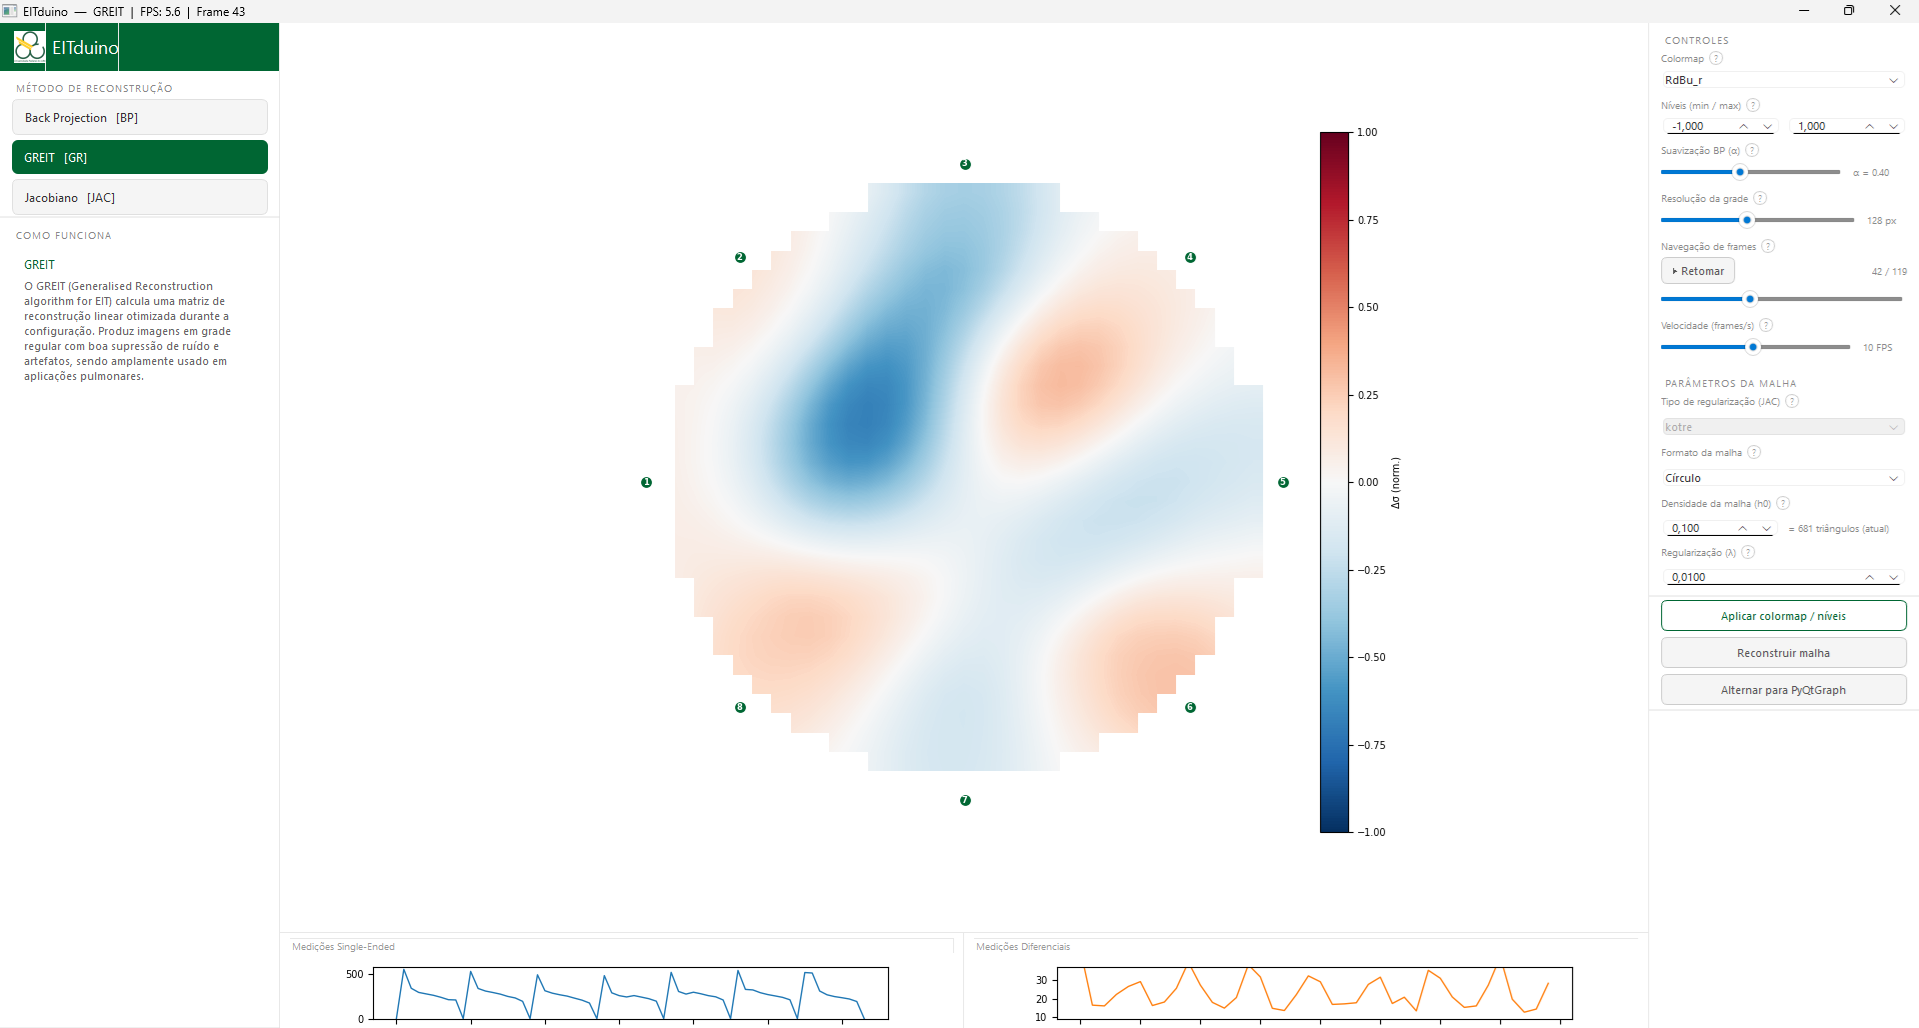
\includegraphics[width=0.85\textwidth]{pictures/GREIT_pyQT_Reg0_01.png}
    \caption{Reconstrução obtida com o método GREIT no \textit{frame} 43, utilizando \(\lambda = 0{,}01\).}
    \label{fig:greit_reg_001}
\end{figure}

\begin{figure}[htbp]
    \centering
    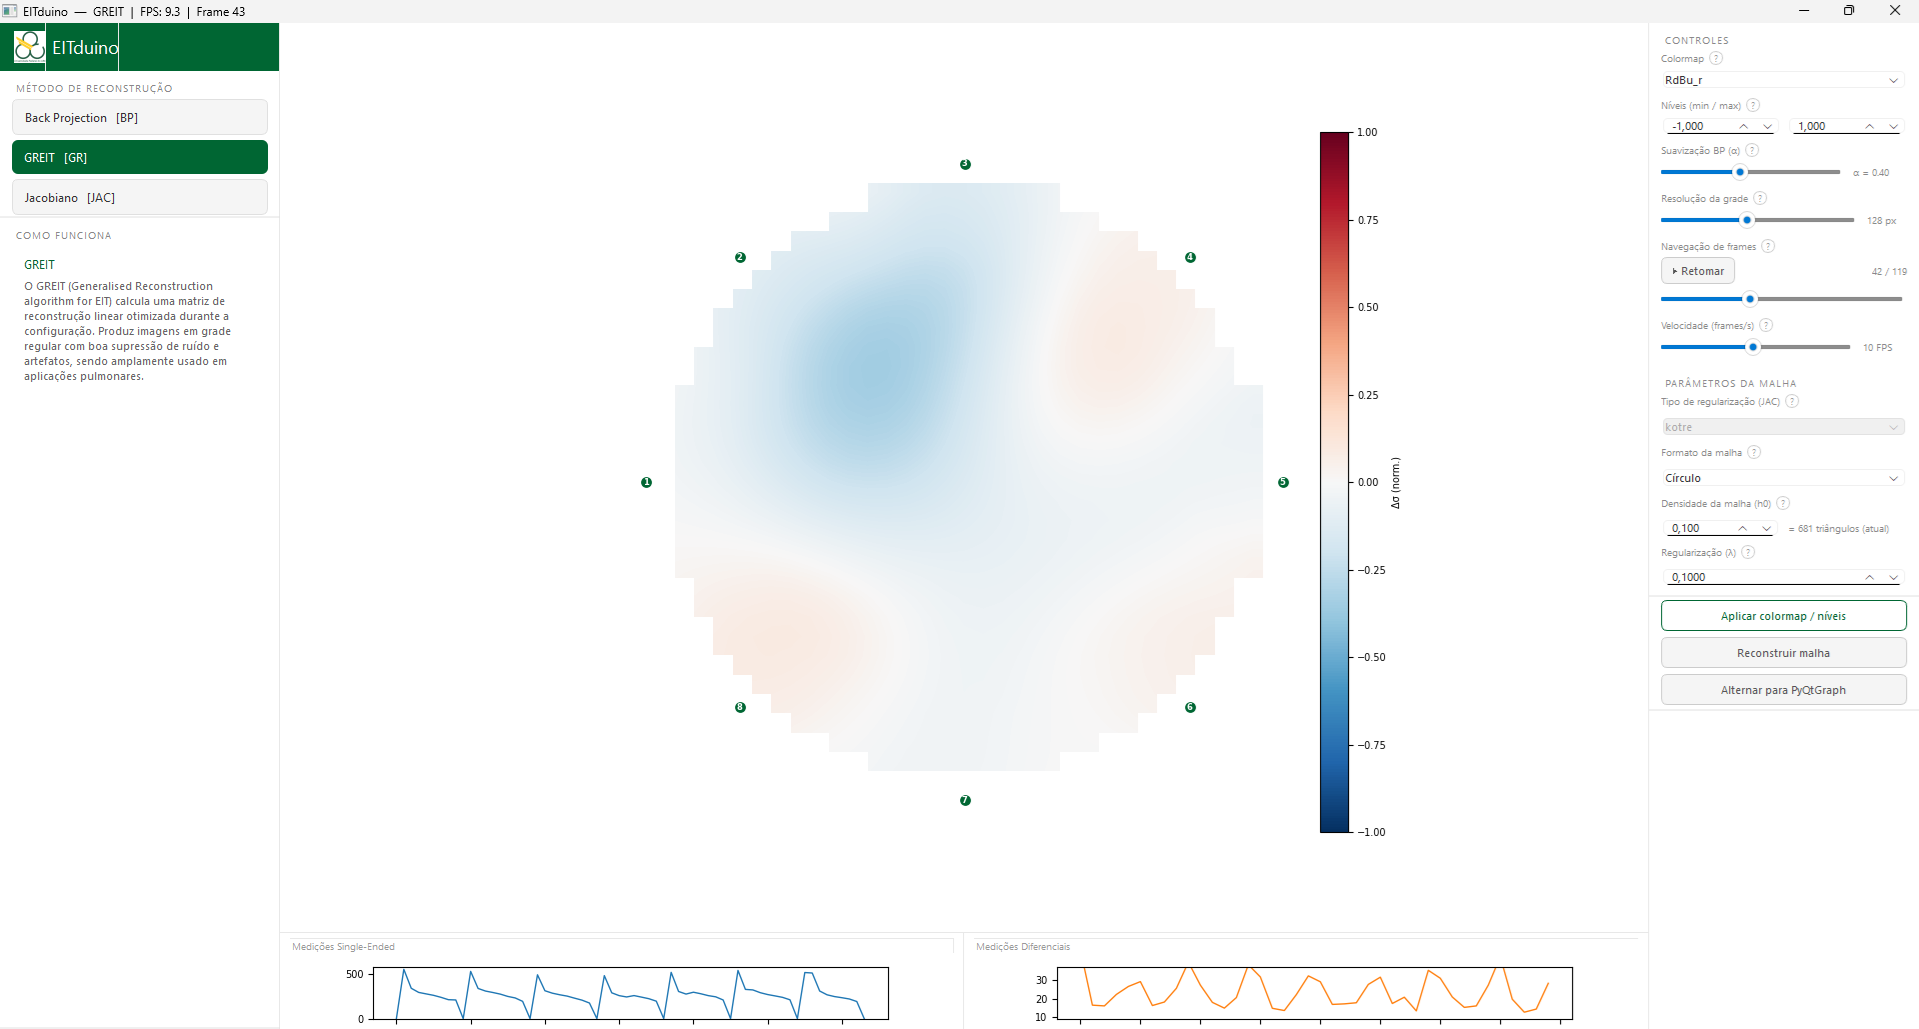
\includegraphics[width=0.85\textwidth]{pictures/GREIT_pyQT_Reg0_1.png}
    \caption{Reconstrução obtida com o método GREIT no \textit{frame} 43, utilizando \(\lambda = 0{,}1\).}
    \label{fig:greit_reg_01}
\end{figure}

\begin{figure}[htbp]
    \centering
    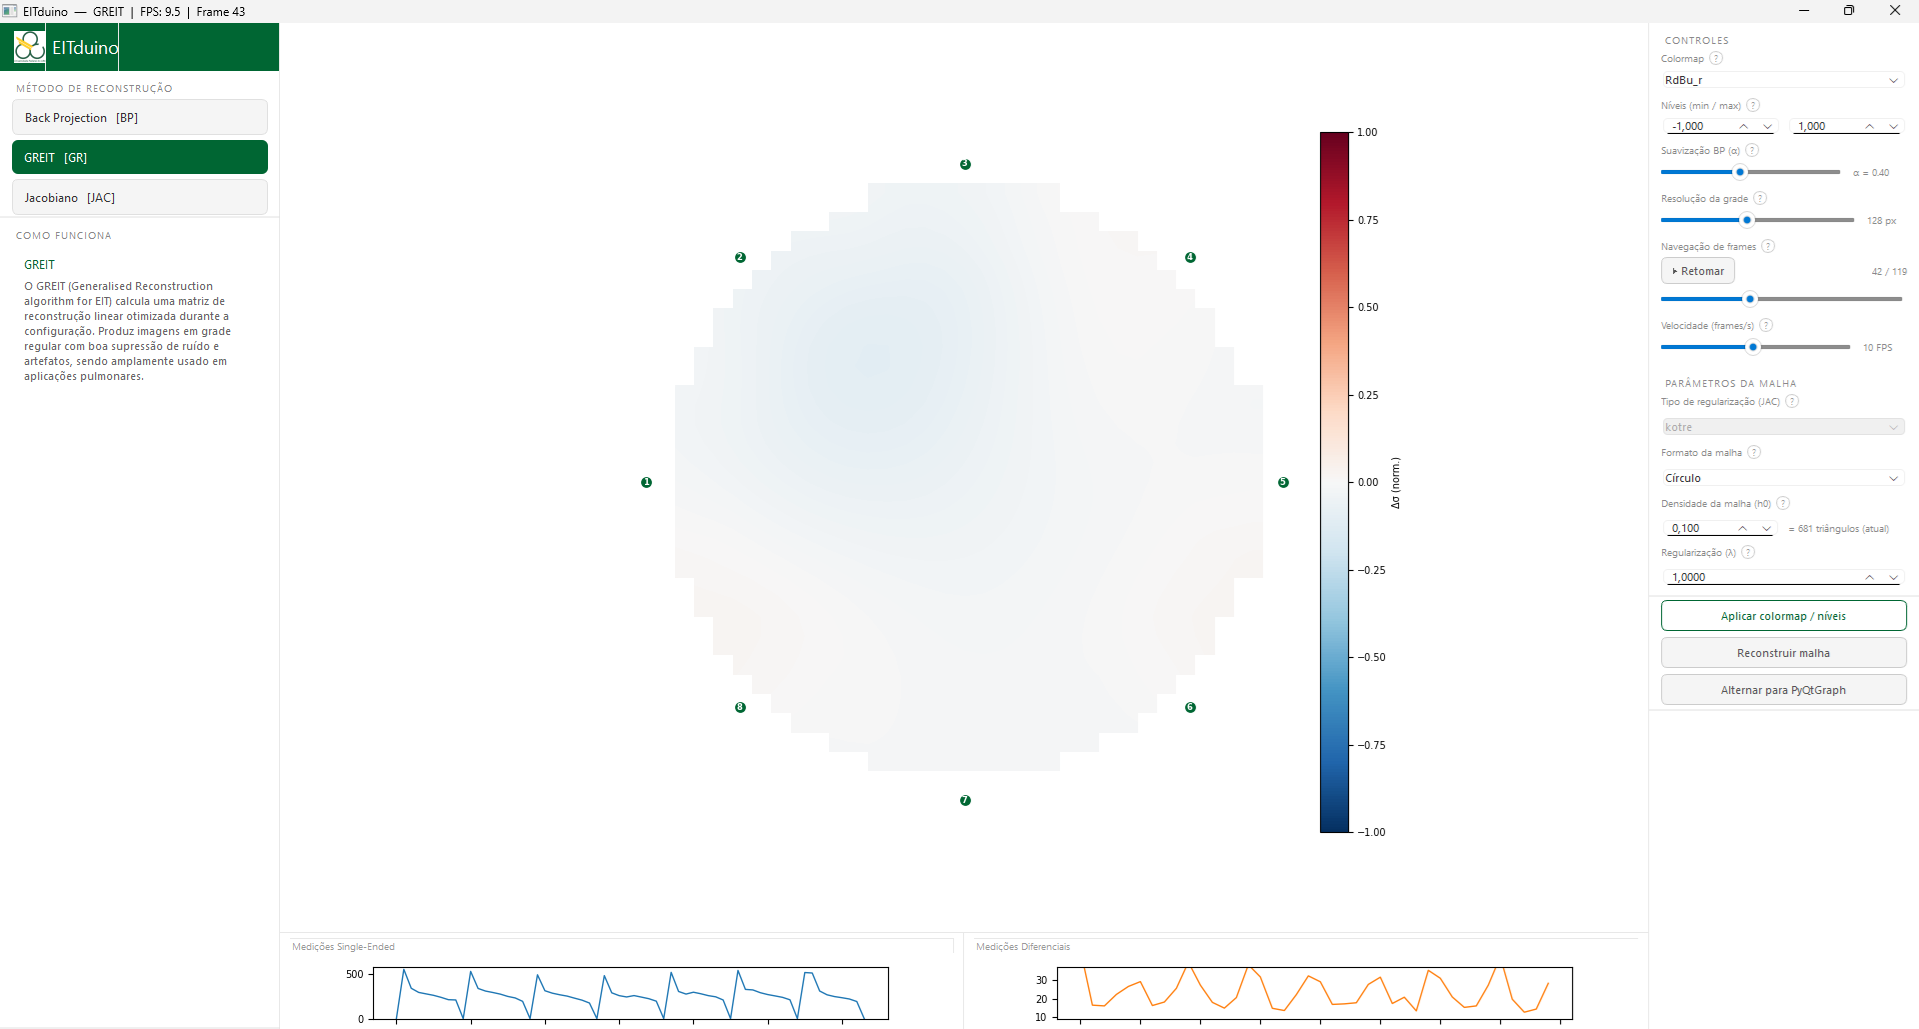
\includegraphics[width=0.85\textwidth]{pictures/GREIT_pyQT_Reg1.png}
    \caption{Reconstrução obtida com o método GREIT no \textit{frame} 43, utilizando \(\lambda = 1{,}0\).}
    \label{fig:greit_reg_1}
\end{figure}

\clearpage

\section{Interface PyQtGraph}
\label{sec:interface_pyqtgraph_resultados}

A interface alternativa desenvolvida com PyQtGraph foi implementada como uma prova de conceito funcional para uma segunda estratégia de visualização das reconstruções. Sua organização foi estruturada em três abas principais: a aba \textit{Solver}, destinada à seleção do método de reconstrução e à exibição de uma descrição resumida do algoritmo ativo; a aba \textit{Controls}, que reúne os parâmetros de visualização e de reconstrução disponíveis nessa implementação; e a aba \textit{Measurements}, voltada à exibição das curvas associadas aos sinais medidos. Em contraste com a interface principal, baseada em uma disposição fixa em painéis, essa versão adota uma organização mais compacta e concentra os controles laterais em abas, preservando os elementos centrais do fluxo de reconstrução. Embora disponha de menos controles do que a interface principal, essa implementação mantém a mesma camada de reconstrução baseada na classe \texttt{EITsolver}. Do ponto de vista arquitetural, a diferença principal está na camada de visualização: a interface em PyQtGraph utiliza \texttt{pg.ImageView} para exibição da imagem reconstruída e \texttt{pg.PlotWidget} para as curvas dos sinais, substituindo o canvas do Matplotlib empregado na interface principal.

\begin{figure}[htbp]
    \centering
    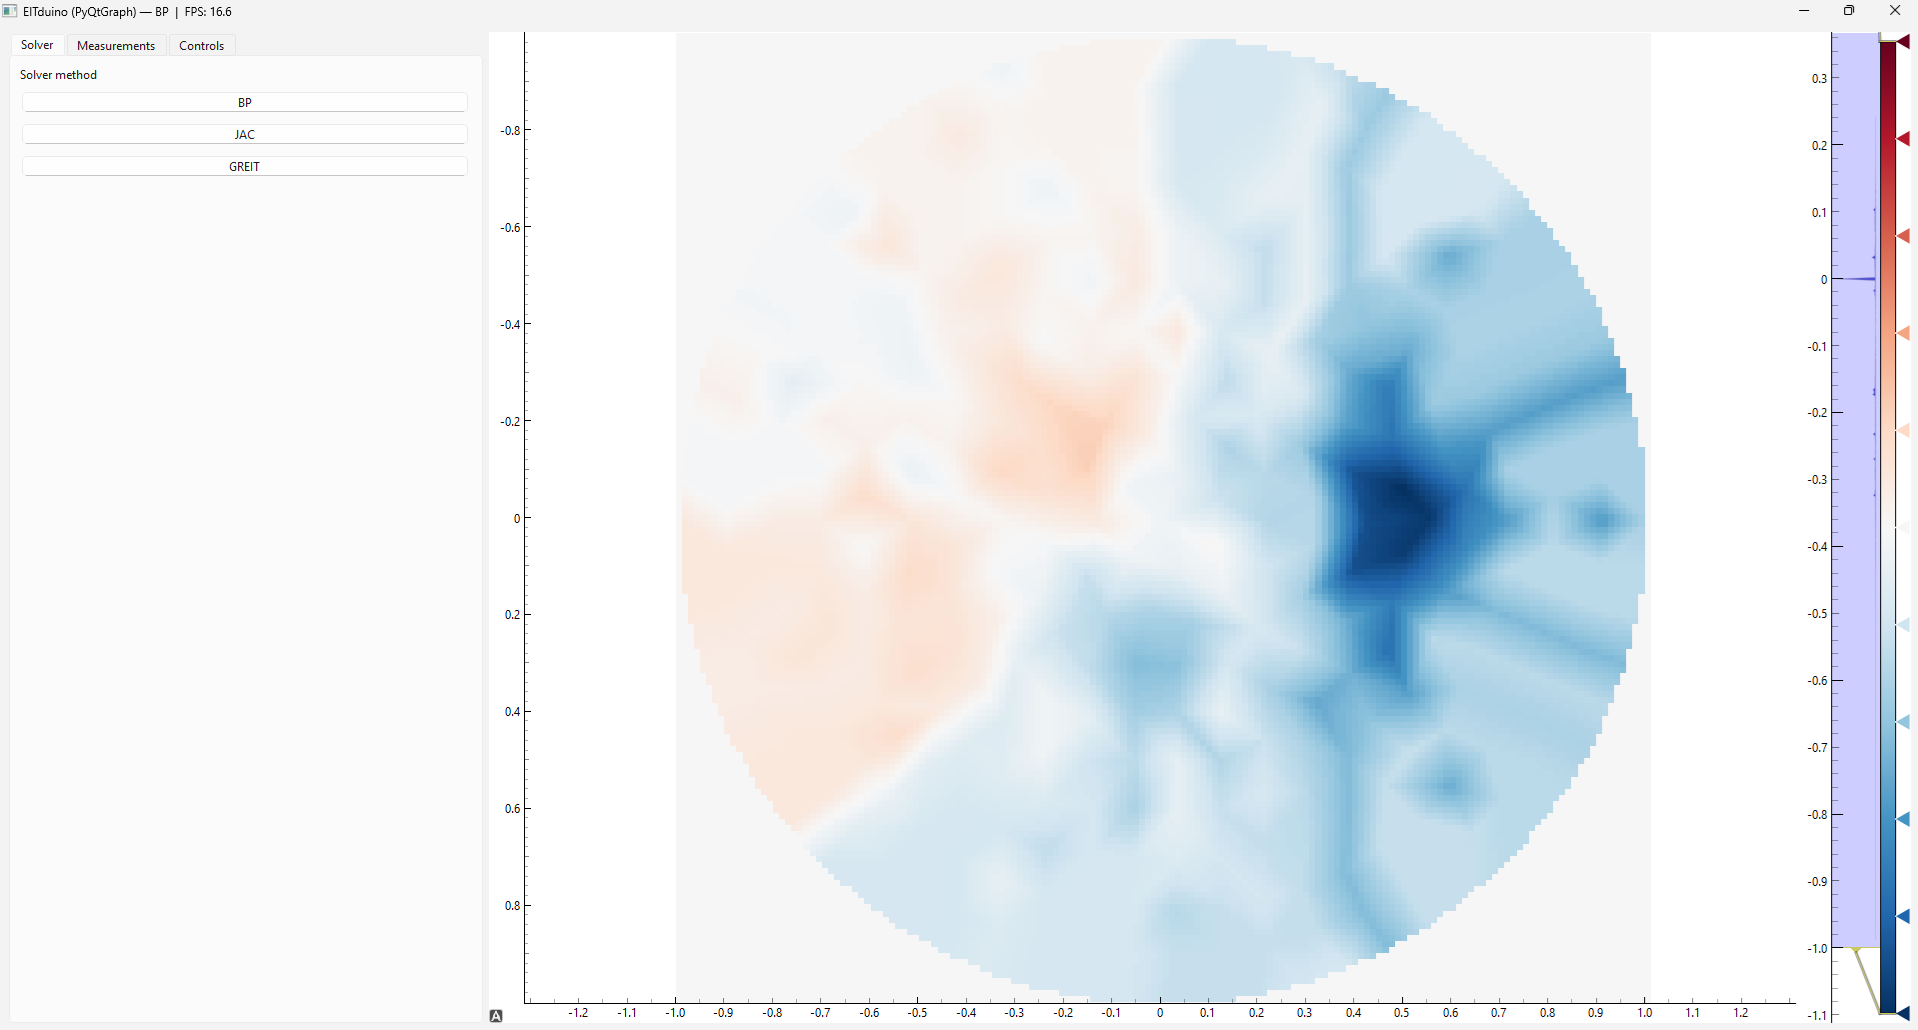
\includegraphics[width=0.85\textwidth]{pictures/BP_PyQtGraph_SolverTab.png}
    \caption{Visão geral da interface alternativa baseada em PyQtGraph, com a aba \textit{Solver} ativa.}
    \label{fig:pyqtgraph_solver_tab}
\end{figure}

\begin{figure}[htbp]
    \centering
    \begin{minipage}{0.48\textwidth}
        \centering
        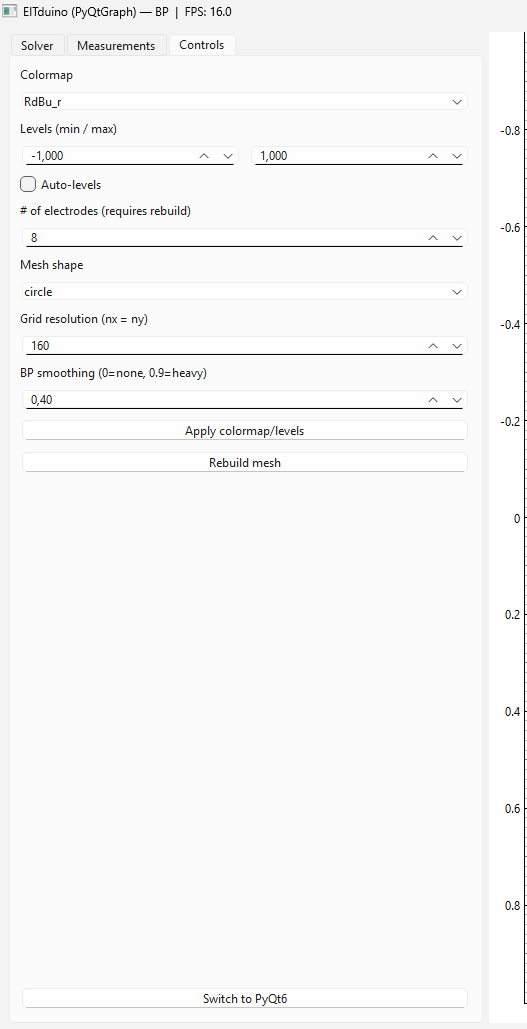
\includegraphics[width=\textwidth]{pictures/BP_PyQtGraph_ControlTab.png}
        \caption*{(a) Aba \textit{Controls}}
    \end{minipage}
    \hfill
    \begin{minipage}{0.48\textwidth}
        \centering
        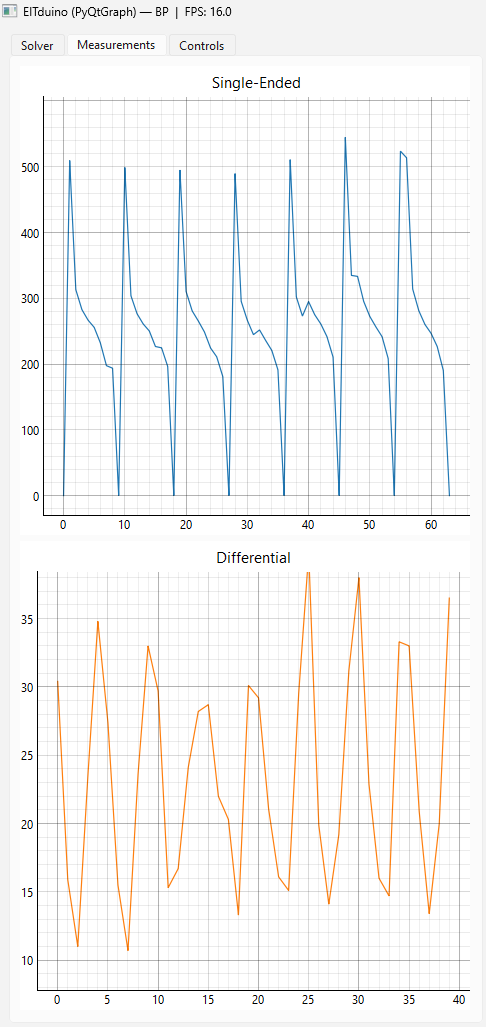
\includegraphics[width=\textwidth]{pictures/BP_PyQtGraph_MeasurementsTab.png}
        \caption*{(b) Aba \textit{Measurements}}
    \end{minipage}
    \caption{Detalhes da interface PyQtGraph com foco nas abas laterais de configuração e visualização dos sinais.}
    \label{fig:pyqtgraph_tabs}
\end{figure}

    % !TEX root = ../raiz.tex

\chapter{Conclusão}

Este projeto é uma forma eficiente e didática de se entender conceitos importantes da TIE e das bibliotecas pyEIT e PyQt, tanto através do tutorial desenvolvido para melhor entender pontos importantes da geração da malha, quanto através da criação da interface em si que representa o ponto principal de pesquisa, visando fornecer uma forma interativa para entender como possíveis alterações de parâmetros podem afetar a imagem gerada.
    
    \printbibliography[heading=bibintoc, title={Referências}]

\end{document}


